\usepackage[authoryear,round]{natbib}
\newcommand{\sheetnum}{%
	02
}
%\setcounter{section}{\sheetnum-3}
\newcommand{\tutorialtitle}{%
    Connectionist Neuron \& Function Fitting
}
\newcommand{\tutorialtitleshort}{%
	Perceptron \& Learning
}
% for slides
\subtitle{\sheetnum \tutorialtitle}

\maxdeadcycles=1000 % Workaround for ! Output loop---100 consecutive dead cycles because of too many figures

% The following use of algroithms does not work well with the notes:
%
%
%
%
% instead use the following for your algorithms:
%
%\begin{figure}[!t]
%\removelatexerror
%\begin{algorithm}[H]
    % your aglo here
    %\label{alg:algolabel}
    %\caption{algocaption}
%\end{algorithm}
%\end{figure}
%\begin{algorithm}
% Below is the definition for the command \removelatexerror:
\makeatletter
\newcommand{\removelatexerror}{\let\@latex@error\@gobble}
\makeatother{}

\begin{document} %%%%%%%%%%%%%%%%%%%%%%%%%%%%%%%%%%%%%%%%%%%%%%%%%%%%%%%

\maxdeadcycles=1000 % Workaround for ! Output loop---100 consecutive dead cycles because of too many figures

\sheet{\sheetnum}{\tutorialtitleshort}

\ttopic{\tutorialtitle}

\columnratio{0.2,0.8}\textbf{}
\begin{paracol}{2}
%\setlength{\columnseprule}{0.1pt}
%\setlength{\columnsep}{5em}

\begin{rightcolumn}

% notes version will ignore it
\begin{frame}
\titlepage
\end{frame}

\begin{frame}{The plan for today}
\tableofcontents
\end{frame}

%\mode<all>
%\section{Connectionist Neuron (Perceptron)}

\begin{frame}\frametitle{\secname}

A neuron is a computational unit for processing information. 

\question{What does a connectionist neuron compute?}\\

\pause
- A connectionist neuron is a type of neuron model which measures for a feature within an observation (a data point). It is a feature detector/extractor e.g. edge detector, above or below a threshold.

\end{frame}

\begin{frame}
A connectionist neuron's response to 1D data:

\begin{figure}[ht]
     \centering
     \savebox{\imagebox}{
	 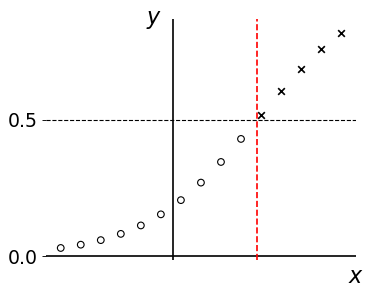
\includegraphics[width=0.3\textwidth]{img/neuron_1d_sigmoid.png}}%
     \begin{subfigure}[t]{0.35\textwidth}
         \centering
         \usebox{\imagebox}% Place largest image
         \caption{}
         \label{fig:neuron_1d_sigmoid}
     \end{subfigure}
     \hspace{10mm}
     \begin{subfigure}[t]{0.35\textwidth}
         \centering
         \raisebox{\dimexpr.5\ht\imagebox-.5\height}{% Raise smaller image into place
         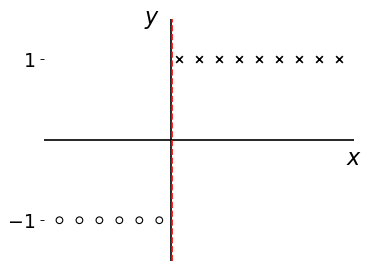
\includegraphics[width=0.9\textwidth]{img/neuron_1d_sign.png}
         }
         \caption{}
         \label{fig:neuron_1d_sign}
     \end{subfigure}
     \mode<article>{
     \caption{Examples of different neuron responses to scalar input of two types: $\times$ and $\circ$. In \ref{fig:neuron_1d_sigmoid}: The neuron's response $y$ is continuous. In \ref{fig:neuron_1d_sign} the neuron repsonse is $+1$ for positive input and $-1$ otherwise. The red lines act as a decision boundary.}
	 }
	 \label{fig:neuron_1d}
\end{figure}

\end{frame}

\begin{frame}\frametitle{
A connectionist neuron's response to 3D data:}

\begin{figure}[ht]
     \centering
	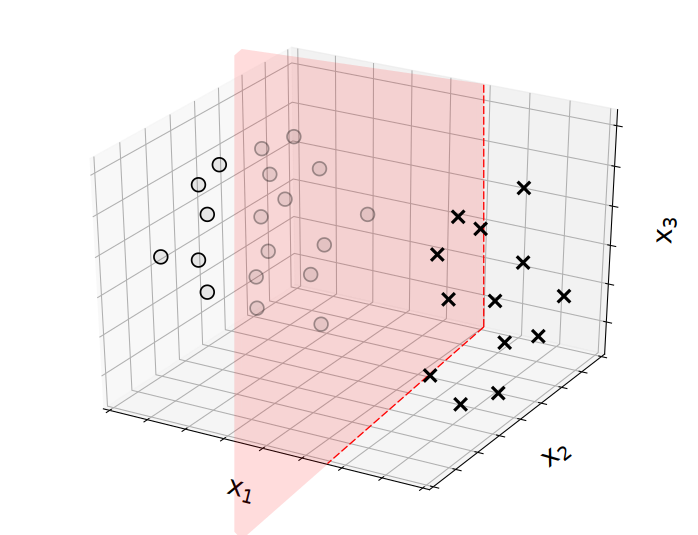
\includegraphics[width=0.4\textwidth]{img/neuron_3d_grid}
     \mode<article>{
	\caption{Examples of a neuron's response to 3D input of types $\times$ and $\circ$. Inputs of different types fall on opposite sides of a plane. The red plane acts as a decision boundary}
	}
	\label{fig:neuron_3d_grid} 
\end{figure}
\end{frame}

\subsection{Components of the connectionist neuron}
    
\begin{frame}
    
    \begin{figure}[h]
        \centering
        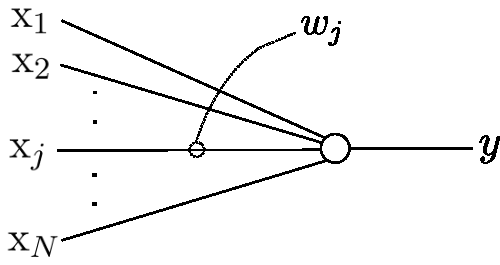
\includegraphics[height=2.5cm]{img/linearNeuron_y.pdf}
        \caption{The input-output relationship for a connectionist neuron. $w_{j}$ describes the connection from the $j$-th input.}
        \label{fig:neuron_diagram}
    \end{figure}
    \notesonly{
    \figref{fig:neuron_diagram} is a diagram of a connectionist neuron.} Given an input vector $\vec x \in \R^{N}$ with components $x_{j}$,
    the connectionist neuron is composed of the following elements:

    \begin{enumerate}[(a)]
        \item weights $\vec w \in \R^{N}$\notesonly{: The weights represent the strength of the connections between the neuron and each component of the input it receives.}\\
        \item A linear filter: \notesonly{Summation of the weighted inputs, i.e. scalar product: }$\vec w^{\top} \vec x = \sum_{j} w_{j} x_{j}$.
        \item A bias value $\theta \in \R$ also known as the \emph{threshold} of the neuron.
        \item An activation function or transfer function $f: \R \mapsto \R$. \\
        \mode<article>{
        
        $f(\cdot)$ controls the range of the neuron's response. It can have the effect of squashing the response to a specific range of values or a specific set of values and preventing other value ranges.
        }
        \item The scalar output of the neuron: $y$.
    \end{enumerate}
    
    \question{How does one interpret the scalar product $\vec w^\top \vec x$?}\\
    
    \mode<article>{
    The scalar product (dot product) acts as measure of similarity between $\vec w$ and $\vec x$.
    By looking at the geometric interpretation of the scalar product (dot product):
    \begin{equation}
    \vec w\top\vec x = ||\vec w||\;||\vec x||\,\cos{\beta}
    \end{equation}
    
    where $\beta$ is the angle between the two vectors. Therefore, $\vec w^\top \vec x$:
    
    \begin{itemize}
    \item is maximal when both vectors point in the same direction.
    \item It is zero if both vectors are orthogonal.
    \item It is maximally negative when both vectors point in opposite direction.
    \end{itemize}
    }
   
\end{frame}
\begin{frame}
    
    \begin{figure}[h]
        \centering
        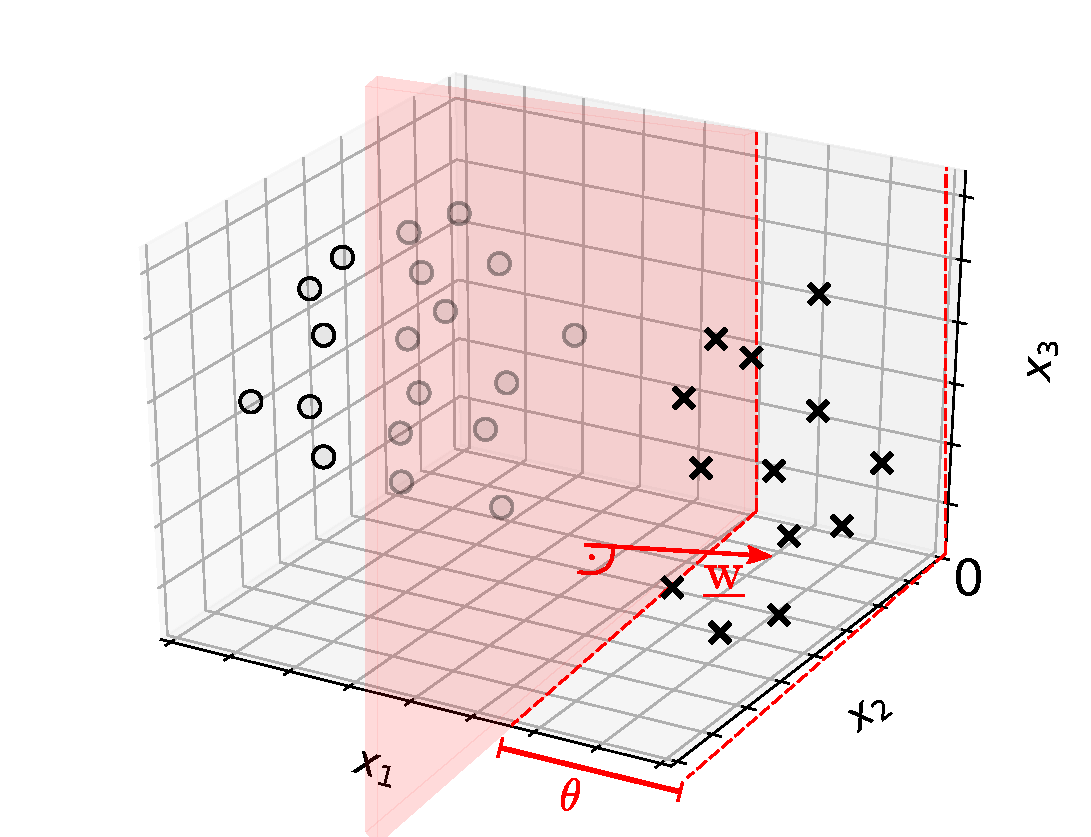
\includegraphics[height=6cm]{img/neuron_3d_grid_hyperplane.pdf}
        \caption{The plane divides the responses of the neuron. In the context of classification it is referred to as the decision boundary.}
        \label{fig:neuron_3d_grid_hyperplane}
    \end{figure}
    
\end{frame}
\begin{frame}
    
    The input-output relationship is described by a linear filter with a static non-linearity $f(\cdot)$:

    \begin{equation}
        \label{eq:linearNeuron}
        y = f \Big(\; \underbrace{\sum_{j=1}^{N} {w}_{j} 
            {x}_j - \theta}_{=:h} \; \Big)
            = f \big(\;  \vec{w}^{\top}
            \vec{x}- \theta \; \big)
            = f(\,h\,)
    \end{equation}
    
	\[ \begin{array}{ll} 
		\vec{x}: & \text{input vector with components } \mathrm{x}_j \\
		y: & \text{scalar output of the neuron } \\
		\vec{w}: & \text{weight vector of the neuron with components }
			\mathrm{w}_{j}\\
		\theta: & \text{threshold of the neuron} \\
		h: & \text{total input of the neuron. } \\
		&\quad h \propto \frac{\vec w^\top \vec x}{\;||\vec w||_2} \text{ component of $\vec x$ in the direction of $\vec w$}\\
		f(\cdot): & \text{transfer function}
	\end{array} \]
    
\end{frame}

\begin{frame}

\question{What roles do the weights and bias play?}

\pause
{}
\mode<article>{
\begin{itemize}
\item[-] $\vec w$ is effectively the normal vector of the hyperplane $\color{red}H = \{\vec x : \vec w^{\top} \vec x = \theta\}$. Therefore, the weights represent the orientation of the hyperplane (see. \figref{fig:neuron_3d_grid_hyperplane}).
\item[-] $\theta$ represents the shift of the hyperplane (see. \figref{fig:neuron_3d_grid_hyperplane}). It is the absolute position of the hyperplane fron the origin along $\vec w$. For any point $\widetilde{\vec x} \in H$ (i.e. points on the plane): 
$\frac{\vec w^\top \widetilde{\vec x}}{\,||\vec w||_2} = \frac{\theta}{\,||\vec w||_2}$
\end{itemize}
}

\mode<presentation>{
    \begin{figure}
        \centering
        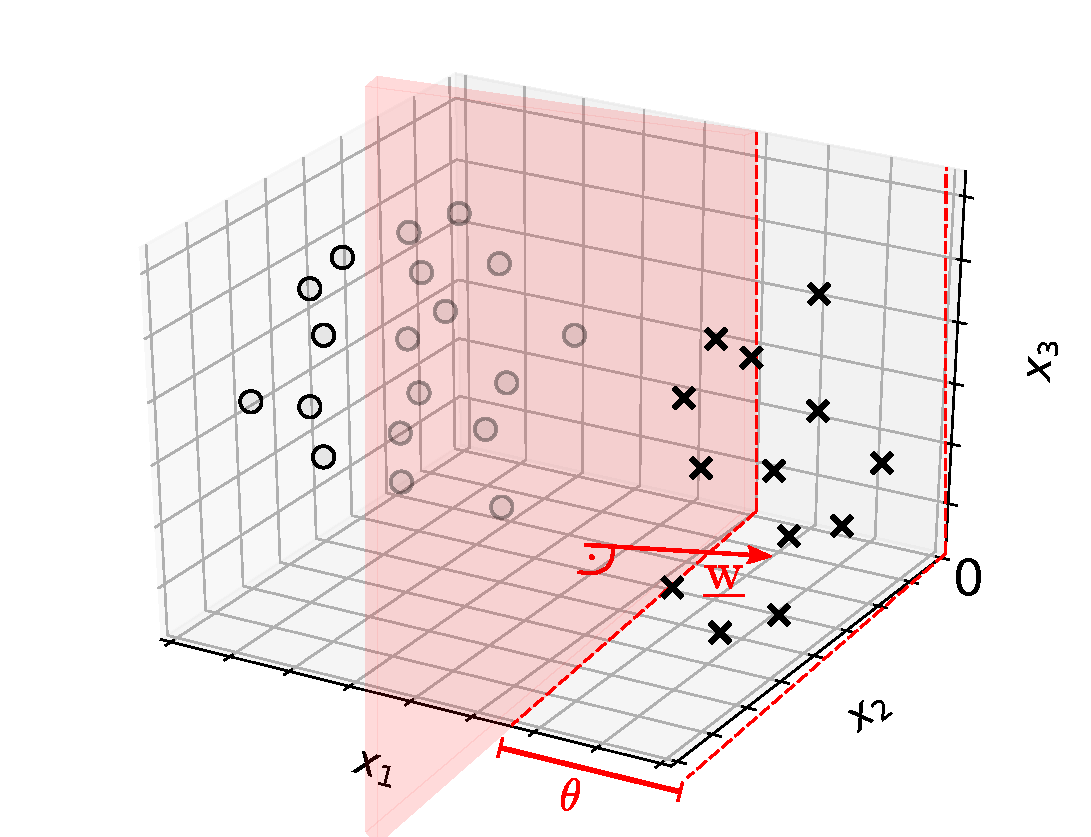
\includegraphics[height=6cm]{img/neuron_3d_grid_hyperplane.pdf}
    \end{figure}
}
\end{frame}

\subsection{Linear vs. non-linear transfer functions}

\begin{frame}


\question{What are the advantages of using a non-linear transfer function instead of a linear one?}

\begin{figure}[ht]
     \centering
     \savebox{\imagebox}{
	 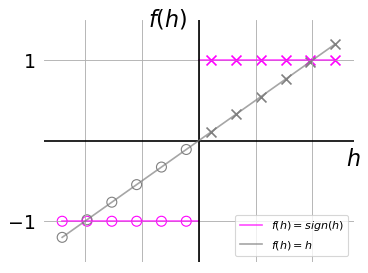
\includegraphics[width=0.3\textwidth]{img/neuron_1d_sign_and_linear}}%
     \begin{subfigure}[t]{0.35\textwidth}
         \centering
         \usebox{\imagebox}% Place largest image
         \caption{\footnotesize Linear vs. non-linear activation}
         \label{fig:linear_sign}
     \end{subfigure}
     \hspace{2mm}
     \begin{subfigure}[t]{0.35\textwidth}
         \centering
         \raisebox{\dimexpr.5\ht\imagebox-.5\height}{% Raise smaller image into place
         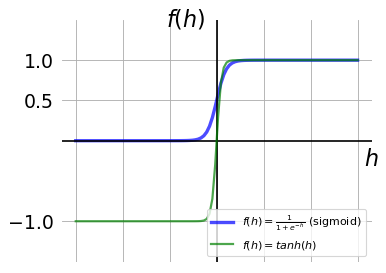
\includegraphics[width=0.9\textwidth]{img/neuron_1d_sigm_tanh}
         }
         \caption{\footnotesize logistic sigmoidal $\scriptstyle f(h)=\frac{1}{1+e^{-h}}$ vs. tanh}
         \label{fig:sigmoid_tanh}
     \end{subfigure}
     \mode<article>{
     \caption{Comparing linear with non-linear activation functions and differentiable alternatives to the sign function.}
     }
	 \label{fig:transfer_linear_nonlinear}
\end{figure}

\pause
- Advantages:
\begin{enumerate}
\item binary classification, either $f(h) \in \{0,1\}$ or $f(h) \in \{-1,1\}$
\item interpret $f(h)$ as a probability. The logistic sigmoidal where $f(h) = \frac{1}{1+exp(-h)}$ yields values in the range of (0,1). The logistic sigmoidal can also be obtained by shifting and scaling the tanh function (see \sectionref{sec:tanh_to_sigmoid}.
\item a multilayer perceptron with only linear transfer functions can be reduced to a single layer. The hidden layers become redundant \footnote{Recent literature reveals interesting insights in what kind of representations are found across the layers of linear networks. For more information see Saxe, A. M., McClelland, J. L., \& Ganguli, S. (2019). A mathematical theory of semantic development in deep neural networks. Proceedings of the National Academy of Sciences, 116(23), 11537-11546.}:\\

     \begin{tabular}{c c c }
     		\raisebox{-9mm}{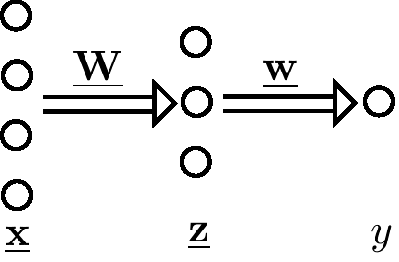
\includegraphics[height=2.25cm]{img/section1_fig16.pdf}}
     	& 
     		\begin{minipage}{10mm}
     			\vspace{10mm}
     		\end{minipage} 
     	& 
     		\parbox{4cm}{
		    \begin{eqnarray*}
		      y & = & \vec{w}^\top \vec{z}  
		      \quad = \quad \vec{w}^\top \vec{W} \, \vec{x} \\
		      & = & (\underbrace{\vec{W}^\top \vec{w}}_{=: \widehat{\vec{w}}})^\top \vec{x}
		      \quad = \quad \widehat{\vec{w}}^\top \vec{x}\\ 
		      & \corresponds & \text{connectionist neuron}
		    \end{eqnarray*}}
	\end{tabular}
\end{enumerate}


\end{frame}

\begin{frame}

\question{How does the logistic sigmoidal function relate to the tanh function?}

\mode<presentation>{

	\only<1,2>{\placeimage{9.5}{4}{img/neuron_1d_sigm_tanh}{width=4.cm}}
}

\mode<article>{

We observe in \figref{fig:sigmoid_tanh} that the logistic sigmoidal function (sigmoid) function is a shifted and scaled variant of the tanh function.
}

From this follows:
	\begin{align}
	f_{{\text{sigmoid}}}(h) 
    & = \frac{1}{1 + e^{-h}} \\
	& = \frac{e^{\frac{h}{2}}}{e^{\frac{h}{2}} + e^{-\frac{h}{2}}} \\
	& = \frac{1}{2} \Bigg(
		\underbrace{\frac{e^{\frac{h}{2}} - e^{-\frac{h}{2}}}{
			e^{\frac{h}{2}} + e^{-\frac{h}{2}}}}_{
				= \tanh \frac{h}{2}}
		+ \underbrace{\frac{e^{\frac{h}{2}} + e^{-\frac{h}{2}}}{
				e^{\frac{h}{2}} + e^{-\frac{h}{2}}}}_{= 1}
		\Bigg) \\
	& = \frac{1}{2} \left( \tanh \frac{h}{2} + 1 \right)
	\end{align}

    
\end{frame}

\subsection{Shortcut notation for weights and bias}

\begin{frame}

\mode<article>{
The bias is effectively a connection between the neuron and an input that is always on. 
We can absorb the bias into the weight vector by prepending it to $\vec w$ and prepending $\vec x$ with an element $x_0 = 1$:
}

    \begin{figure}[h]
        \centering
        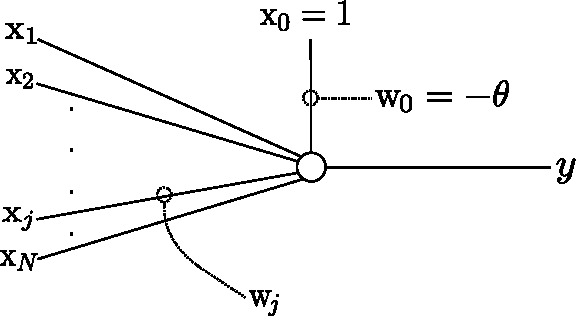
\includegraphics[height=3cm]{img/section1_fig6}
         \caption{Absorb bias into weight vector.}
         \label{fig:weight_with_bias}
    \end{figure}
 
\only<1>{
\mode<article>{   
The response of the neuron depicted in \figref{fig:weight_with_bias} can be computed by:
}

\begin{equation}
	y = f\big( \sum_{{\color{blue}j=0}}^{N} \mathrm{w}_j \mathrm{x}_j \big)
		= f( \vec{w}^\top \vec{x} )
	\label{eq:weight_with_bias}
\end{equation}

\mode<article>{

Note that the sum in \eqref{eq:weight_with_bias} now iterates from ${\color{blue}j=0}$ instead of $j=1$ as was done in \eqref{eq:linearNeuron} in order to include the bias element.
}

}

\only<2>{


	$\vec{w}$ will be used for $\rmat{ \mathrm{w}_1 \\ \vdots\;\,\\ \mathrm{w}_N}$ 
	as well as for $\rmat{ \mathrm{w}_0 \\ \mathrm{w}_1 \\ \vdots\;\, \\ \mathrm{w}_N}$. \\
	
	\rule{2cm}{0pt}
	
	Accordingly,
	$\vec{x}$ will be used for $\rmat{ \mathrm{x}_1 \\ \vdots\;\,\\ \mathrm{x}_N}$ 
	as well as for $\rmat{ \mathrm{x}_0 \\ \mathrm{x}_1 \\ \vdots\;\,\\ \mathrm{x}_N}$.
	
	\mode<article>{
	Whether the bias is absorbed or not should become apparent from the context or explicitly from the limits of the sum.
	}
}

\end{frame}

%\mode*

%\clearpage

%\mode<all>
%\section{Limitations of Perceptrons}

\mode<presentation>{
\begin{frame} 
    \begin{center} \huge
        \secname
    \end{center}
    \begin{center}
    From neurons to neural networks
    \end{center}
\end{frame}
}

\mode<article>{
Connectionist neurons, or perceptrons, are limited in the variety of functions they are able to fit. 
When dealing with classification problems, a perceptron can only find a linear separation between any two classes. Irrespective of the neuron's non-linear activation function, the perceptron is regarded as a \emph{linear classifier}. Whether something falls on one side of the decision boundary or the other, is entirely based on applying a linear filter (i.e. $\vec w^{\top} \vec x$). The non-linearity $f(h)$ merely controls the value range of the neuron's response ($\{0,1\}, (-1,+1)$, \ldots) which helps in interpreting the neuron's response.\\

If observations for two different classes are distributed such that one cannot draw a line to separate them, then the two classes
are not linearly separable. In this case, the perceptron will fail to find a suitable classification boundary between the two classes.
}

\begin{frame}\frametitle{Linear classifiers/linear decision boundaries}

Consider the following binary classification problems with $\vec x \in \R^2$.{}

\question{Can you find a line that separates the two classes for each case?}

\begin{figure}[h]
    \centering
	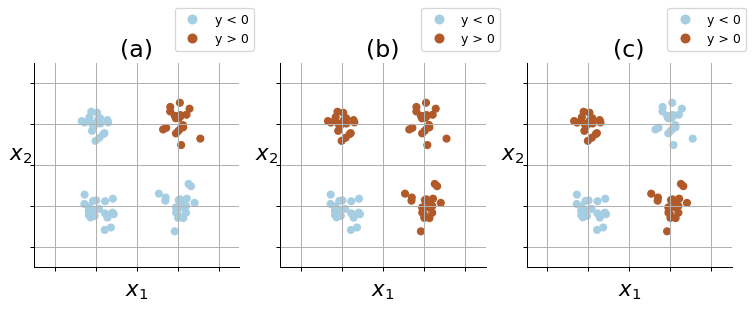
\includegraphics[width=0.8\textwidth]{img/and_or_xor_y}
	\mode<article>{
	\caption{(a) points are classified according to the AND function,
	(b) points are classified according to the OR function,
	(c) points are classified according to the XOR function.
	}
	}
	\label{fig:and_or_xor} 
\end{figure}

\mode<article>{
In \figureref{fig:and_or_xor}, particularly (a) and (b),
it is possible to draw a line that separates the classes. Therefore, the AND and OR functions are linearly separable.
A perceptron is capable of finding such a separating line. However, this does not apply to the third case, for the XOR function.
It is impossible to find a single line that will separate the classes.\\
The XOR function is not linearly separable.
}

\pause 

\question{Can we solve the XOR problem with multiple perceptrons? How?}\\

%\slidesonly{
%\begin{figure}[ht]
     %\centering
	%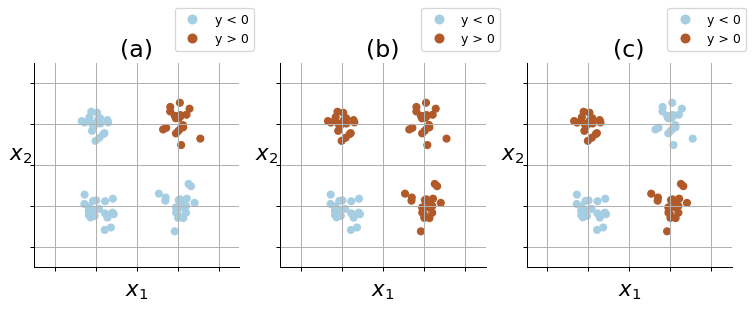
\includegraphics[trim=480 0 0 30, clip, width=0.4\textwidth]{img/and_or_xor_y.png}
	%\caption*{A single perceptron can not solve the XOR problem.}
	%\label{fig:xor} 
%\end{figure}
%}

\pause

\notesonly{
- Yes, think of it as a divide and conquer approach. We split the XOR problem into multiple sub-problems. 
A perceptron is used to solve each sub-problem.

If you're familiar with Boolean algebra, you might recognize the following expression for the XOR function:
}
\mode<presentation>{
\vspace{-10mm}
}

\begin{equation}
\label{eq:xor}
\mathrm{XOR}(x_1, x_2) = 
({\color{magenta}\,{x_1} \; \mathrm{AND} \; \overline{x}_2 \,})
 \;\; \mathrm{OR} \;\; 
({\color{green}\, \overline{x}_1 \; \mathrm{AND} \; x_2 \,})
\end{equation}

\end{frame}

\begin{frame}{Inversion/NOT-Gate}

\begin{center}
\begin{minipage}{0.9\textwidth}

\begin{center}
\begin{minipage}{0.45\textwidth}
	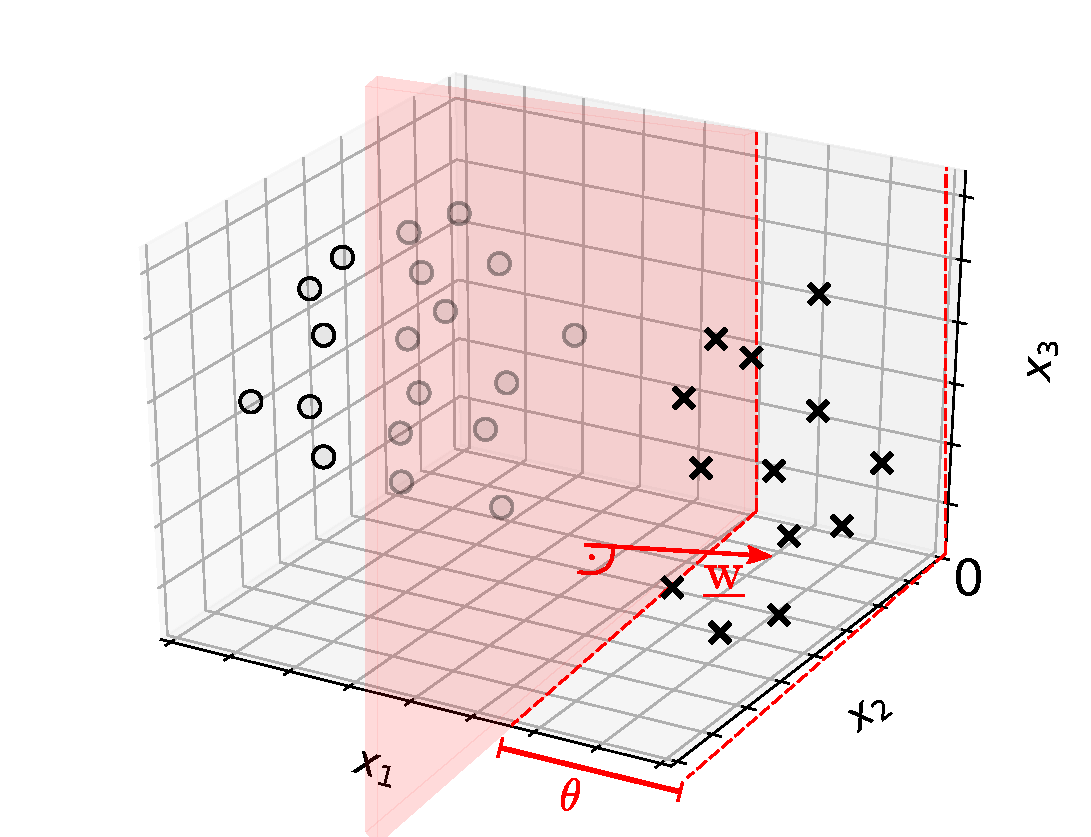
\includegraphics[width=0.9\textwidth]{img/neuron_3d_grid_hyperplane}
\end{minipage}
\begin{minipage}{0.45\textwidth}
	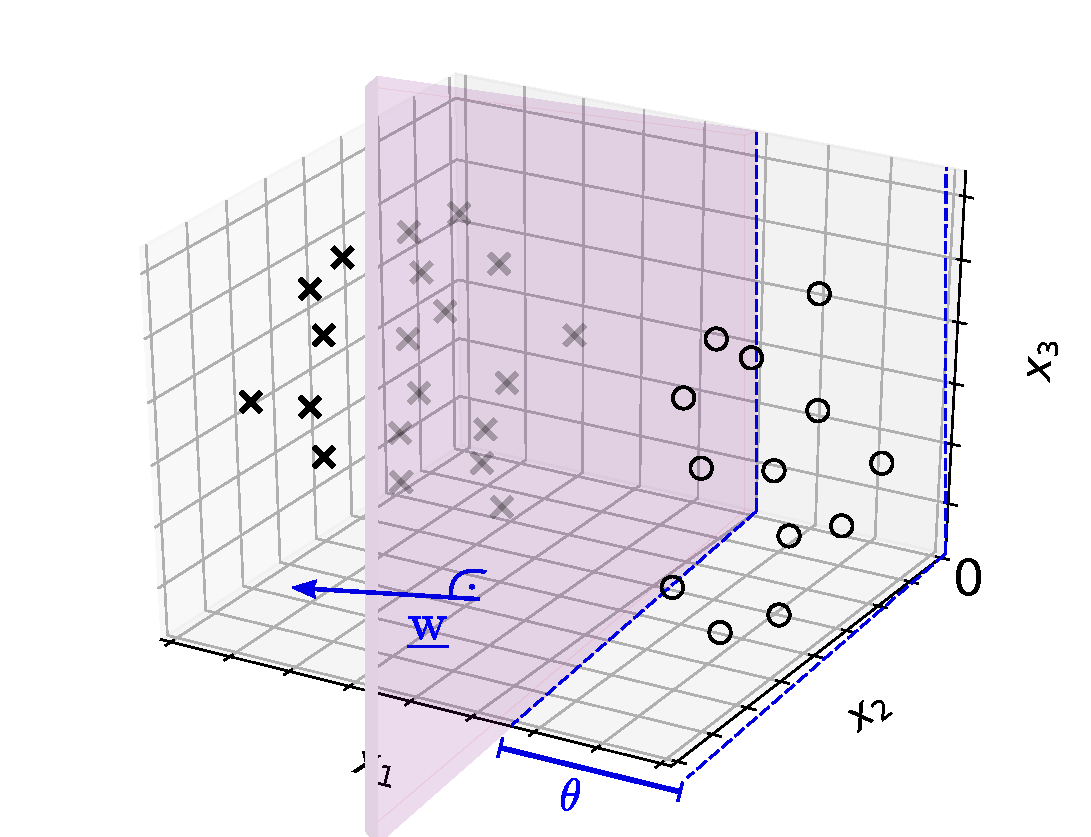
\includegraphics[width=0.9\textwidth]{img/neuron_3d_grid_hyperplane_flip}
\end{minipage}

\end{center}
\end{minipage}
\captionof{figure}{Inverting a neuron's response by flipping the hyperplane}
\end{center}

\end{frame}


\mode<article>{
For instance, the first perceptron ${\color{magenta}s^1_1}$ is tasked to separate the bottom-right cloud of points from the rest. 
A second perceptron ${\color{green}s^1_2}$ is used to separate the top-left cloud from the rest.
A third perceptron ${\color{blue}s^2_1}$ will then use the responses of both and respond to ``is \textbf{only one} of the two perceptrons \textbf{on}?''.

\figref{fig:build_xor} illustrates this approach. One need only recognize that each sub-problem is linearly separable.\\
}

\begin{frame}

\slidesonly{
\begin{equation}
\label{eq:xor}
\mathrm{XOR}(x_1, x_2) = 
({\color{magenta}\,{x_1} \; \mathrm{AND} \; \overline{x}_2 \,})
 \;\; \mathrm{OR} \;\; 
({\color{green}\, \overline{x}_1 \; \mathrm{AND} \; x_2 \,})
\end{equation}
}

\begin{figure}[ht]
    \centering
	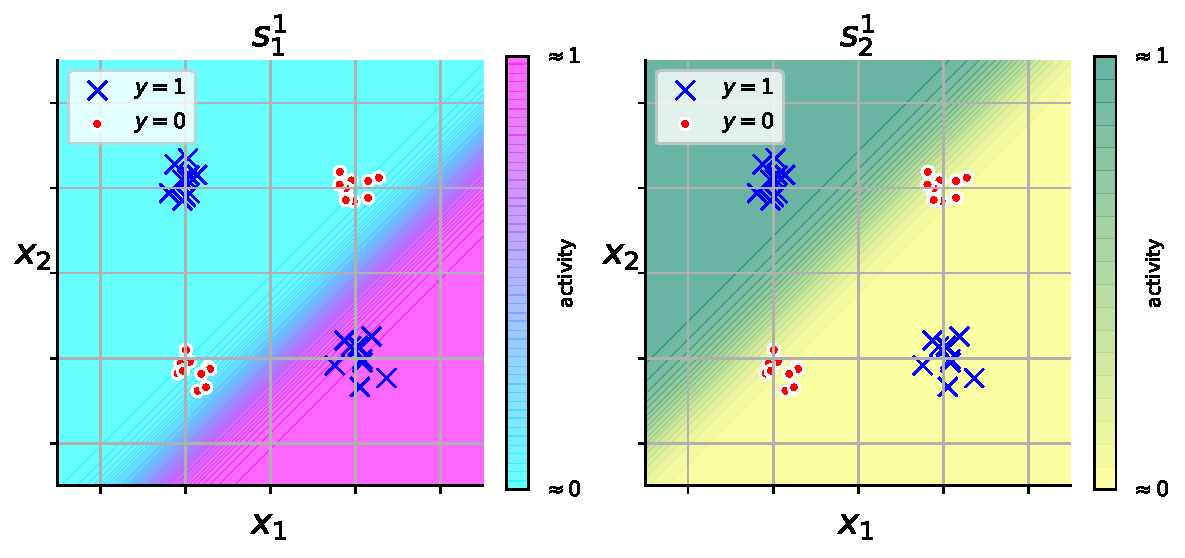
\includegraphics[width=0.75\textwidth]{img/build_xor_crf}
	\caption{Solving sub-problems of the XOR problem.}
	\label{fig:build_xor} 
\end{figure}

\end{frame}

\begin{frame}

\begin{figure}[ht]
    \centering
	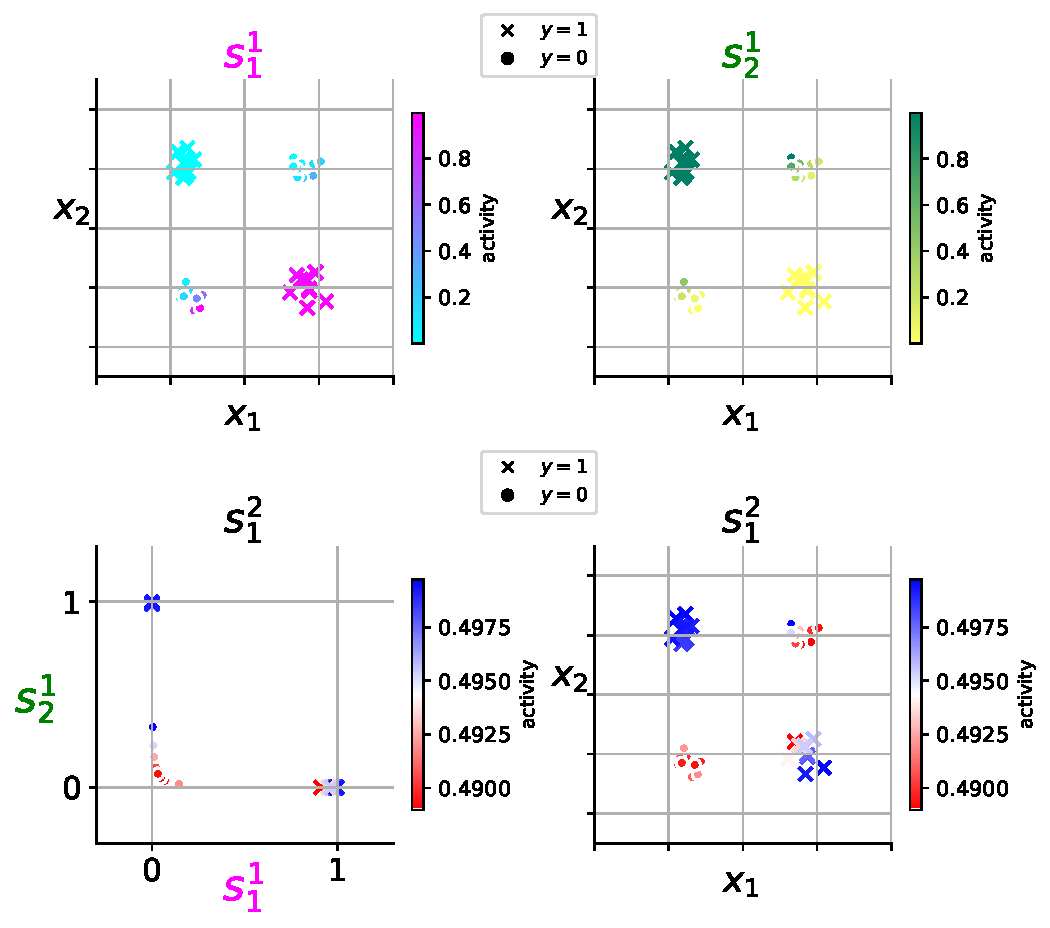
\includegraphics[width=0.75\textwidth]{img/build_xor}
	\caption{Solving sub-problems of the XOR problem.}
	\label{fig:build_xor} 
\end{figure}

\end{frame}


\mode<article>{
\figref{fig:xor_decisions} visualizes the response of the final neuron $s^2_1$ for different values of $x_1$ and $x_2$. The space is partitioned into one region in which the activity is $< 0.5$ and two disjoint regions (top-left \& bottom-right) in which the activity is $> 0.5$.
}

\begin{frame}
\begin{figure}[ht]
     \centering
     \savebox{\imagebox}{
     \mode<presentation>{
	 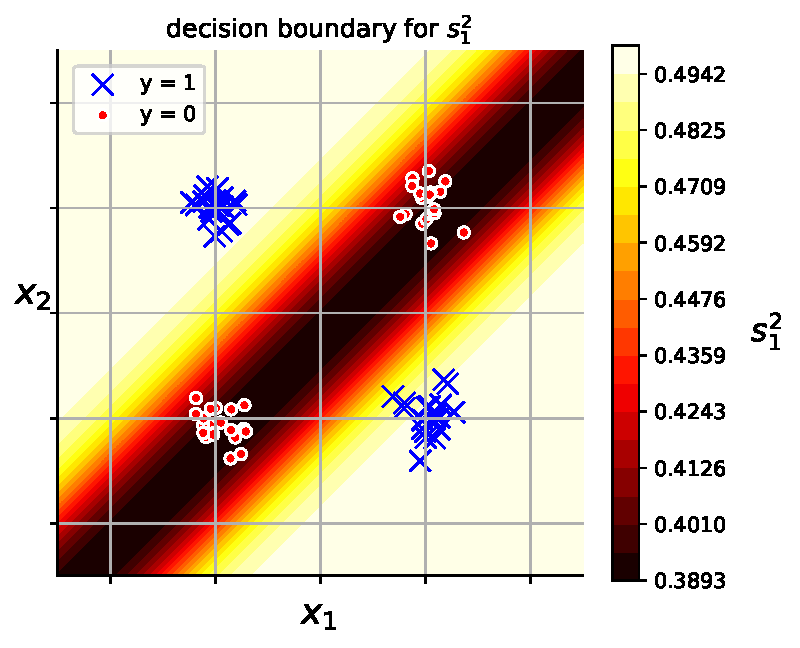
\includegraphics[width=0.4\textwidth]{img/xor_decision}
	 }
     \mode<article>{
	 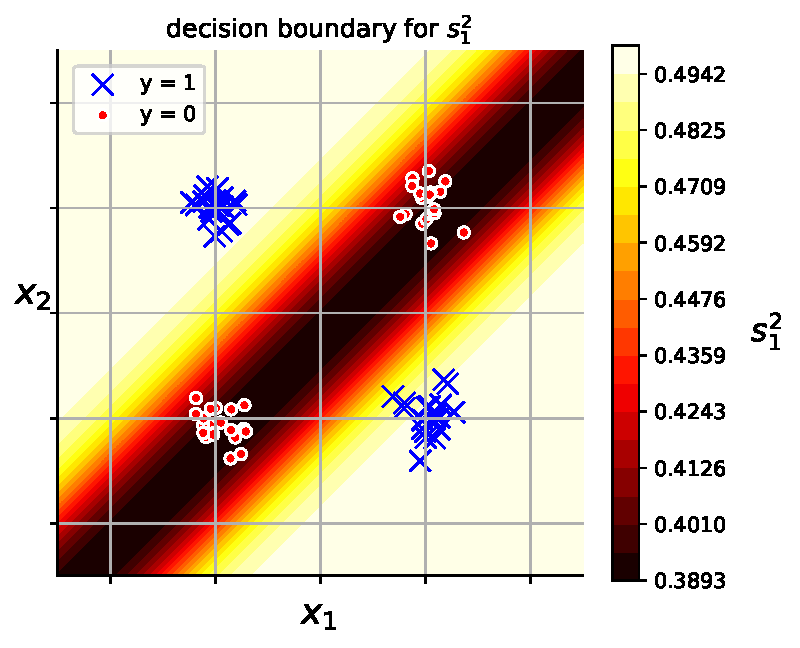
\includegraphics[width=0.35\textwidth]{img/xor_decision}
	 }
	 }%
     \begin{subfigure}[t]{0.35\textwidth}
         \centering
         \usebox{\imagebox}% Place largest image
         \caption{}
         \label{fig:xor_decisions}
     \end{subfigure}
     \slidesonly{
     \hspace{4mm}
     \begin{subfigure}[t]{0.45\textwidth}
     }
    \notesonly{
     \hspace{1mm}
     \begin{subfigure}[t]{0.38\textwidth}
     }
         \centering
         \raisebox{\dimexpr.5\ht\imagebox-.5\height}{% Raise smaller image into place
         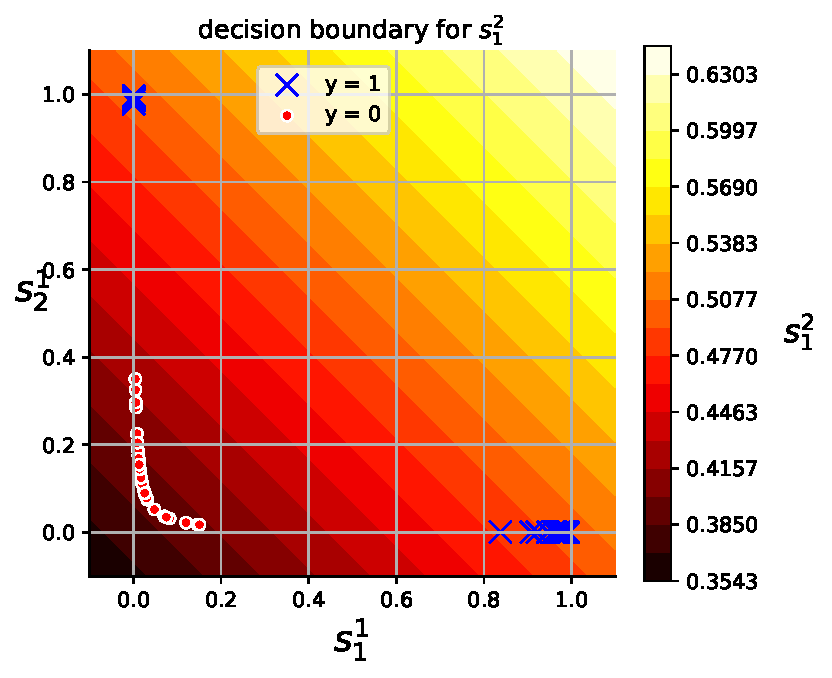
\includegraphics[width=0.9\textwidth]{img/xor_decision_s}
         }
         \caption{}
         \label{fig:xor_decisions_s}
     \end{subfigure}
	\caption{Identifying the decision boundaries.}
\end{figure}
\end{frame}

\newpage
\mode<article>{


What we are essentially describing is a Multilayered perceptron (MLP) with an architecture as illustrated in \figref{fig:xor_mlp_arch}. This MLP is made up of an output layer with a single output neuron ${\color{blue}s^2_1}$, and one hidden layer with two hidden neurons, ${\color{magenta}s^1_1}$ and ${\color{green}s^1_2}$ (the superscript denotes the layer index, the subscript denotes the neuron index within its layer). The terms ``neurons'' and ``nodes'' are treated as synonyms.
}
\begin{frame}

\begin{figure}[ht]
    \centering
	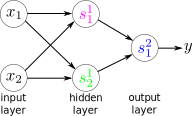
\includegraphics[width=0.4\textwidth]{img/xor_mlp_arch}
	\caption{simplified MLP architecture}
	\label{fig:xor_mlp_arch} 
\end{figure}



\end{frame}



%\mode*

%\newpage

\mode<all>
\section{Ingredients for function fitting}

\mode<presentation>{

\begin{frame}
\begin{center}
    \begin{center} \huge
        \secname
    \end{center}
    
    \begin{center}
		
\includegraphics[width=0.25\textwidth]{img/meme_ingredients}
    \end{center}
    
    \begin{center}
    Tuning the weights of a neural network to perform some task.
    \end{center}
\end{center}
\end{frame}
}

\begin{frame}\frametitle{\secname}

    \mode<article>{
    Fitting an MLP to a desired function $y(\vec x)$ requires the following:
    }

    \begin{enumerate}
    \item 
    \mode<article>{A cost function  with the objective to optimize it, often a minimization problem:}
    \mode<presentation>{A cost function:\vspace{-10mm}}
	\begin{equation}
		e\tyxw \eqexcl \min_{\vec w}
	\end{equation}
    \pause
    \item A performance measure, a criterion for \emph{model selection}.
    \mode<article>{Specifically, \\

    the generalization \textbf{error} $E^G$ which is defined as:}	
    \begin{equation} 
                \EGw \; := \; \left<\,e\,\right>_{y_T, \vec{x}; \vec w} 
                \; = \; \iint d \vec{x} \, dy_T \; 
                    P{(y_T, \vec{x})} \, e{\tyxw}
    \end{equation}
    \pause
    Because $P{(y_T, \vec{x})}$ is not known, \mode<article>{we turn to the principle of empirical risk minimization (ERM).
    According to ERM we can approximate $\EGw$ by computing the} empirical average $\ETw$ using the available training data:
    $$
    \left\{\left(\vec x^{(\alpha)}, y_T^{(\alpha)}\right)\right\}, \alpha=1,\ldots,p
    $$.
    \mode<article>{The training error $\ETw$ becomes:}

    \mode<presentation>{\vspace{-10mm}}
    \begin{equation}
    \text{batch training error:}\quad \ETw=\frac{1}{p}\sum_{\alpha=1}^{p} \underbrace{e\tyxwalpha}_{e^{(\alpha)}}
    \end{equation}
    \mode<article>{
    where $e\tyxwalpha$ (or $e^{(\alpha)}$ for brevity) is the cost computed from the prediction for a specific observation $y(\vec x^{(\alpha)};\vec w)$ and its corresponding label $y_T^{(\alpha)}$. The superscript $^{(\alpha)}$ is used to index a specific point (sample) in the dataset.
    }
    \pause
    \item A model with tunable parameters $\vec w$: MLP, connectionist neuron, \ldots
    \item A learning algorithm\mode<article>{ for finding the set of parameters in our model that will minimize the cost function.\\
    This can be done analytically (depending on some conditions) or through an iterative learning algorithm (e.g. gradient-based learning)}
    \end{enumerate}

\end{frame}


\mode*

\newpage

\mode<all>
\subsection{Cost functions}
\begin{frame}\frametitle{\subsecname}
\mode<article>{
A cost function $e\tyxw$, quantifies the discrepancy between the model's prediction $y(\vec x; \vec w)$ and the label $y_T$ which $\vec x$ is assigned to.
}
Choosing a cost function accounts for 
\begin{enumerate}
\item the type of problem (i.e. regression vs. classification), 
\item how the model is penalized for different types of mistakes it can make such as:
small errors are tolerable, large errors are penalized less, etc.
\end{enumerate}
\mode<article>{
The choice of cost function has a direct effect on how the model learns. For example, we will later see in gradient-based learning how the error function can modulate how fast or slow a model learns.
}
\end{frame}

\subsubsection{Cost functions for Regression}

\begin{frame}\frametitle{\subsecname}

  \begin{tabular}{c c c}
    \parbox{4cm}{
      \[ \underbrace{\vec{x}
          \in \mathbb{R}^N
      }_{\text{feature vector}}
      \longrightarrow 
      \underbrace{y
      \in \mathbb{R}
      }_{\substack{\text{scalar}\\ \text{attribute}}}
      \]}
    & & 
    \parbox{8cm}{\footnotesize
      \begin{tabular}{l l}
	$y_T(\vec x)$: & true value of attribute \\
	$y(\vec{x}; \vec w)$: & predicted value of attribute \\
					& (e.g. by MLP)
      \end{tabular}
    }
  \end{tabular}
     \pause

  \begin{block}{individual cost $e\tyxw$}
    \begin{center} 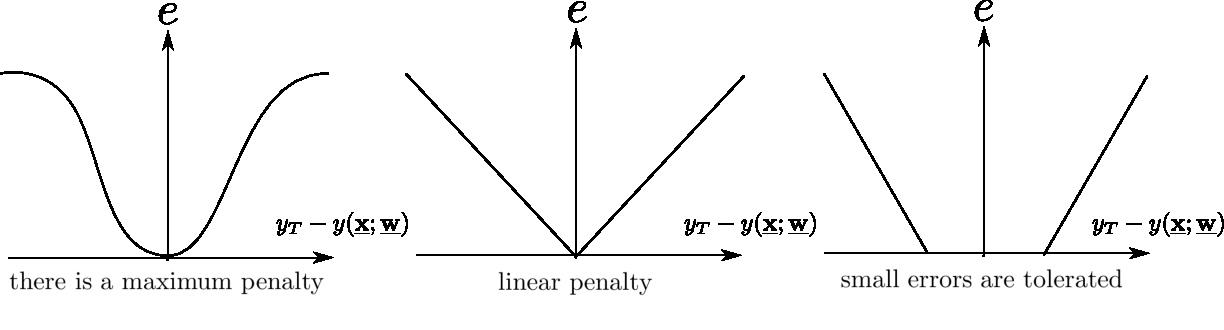
\includegraphics[width=12cm]{img/section1_fig17_v2.pdf} \end{center}
  \end{block}
\end{frame}

\begin{frame}\frametitle{Quadratic vs. linear error}

\begin{figure}[ht]
     \centering
     \savebox{\imagebox}{
	 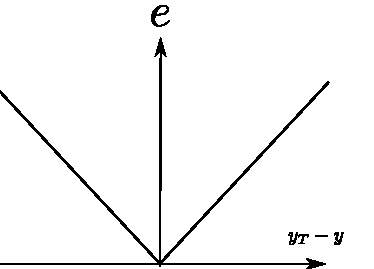
\includegraphics[width=0.4\textwidth]{img/section1_fig17_linear}}%
     \begin{subfigure}[t]{0.45\textwidth}
         \centering
         \usebox{\imagebox}% Place largest image
         \caption{linear error}
         \label{fig:quadratic}
     \end{subfigure}
     \hfill
     \begin{subfigure}[t]{0.45\textwidth}
         \centering
         \raisebox{\dimexpr.5\ht\imagebox-.5\height}{% Raise smaller image into place
         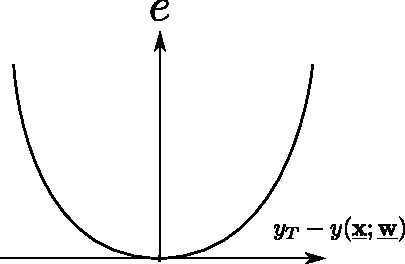
\includegraphics[width=0.99\textwidth]{img/section1_fig17_quadratic}
         }
         \caption{qudratic error}
         \label{fig:linear}
     \end{subfigure}
     \mode<article>{
     \caption{quadratic vs. linear error}
     }
	 \label{fig:quadratic_vs_linear}
\end{figure}


\begin{equation}
e_{\text{quadratic}}\tyxw := \frac{1}{2} \Big( y_{T}(\vec x) - y(\vec x;\vec w)\Big)^{2}
\label{eq:quadratic_error}
\end{equation}

\begin{equation}
e_{\text{linear}}\tyxw := \Big| y_{T}(\vec x) - y(\vec x;\vec w)\Big|
\label{eq:linear_error}
\end{equation}
\mode<article>{
The purpose of having $\frac{1}{2}$ in \eqref{eq:quadratic_error} is for convenience for when we calculate the derivative later. 
Both the quadratic and linear cost functions are symmetric. They therefore yield the same error regardless of the sign. However, the differences between them are:
}
\end{frame}
\begin{frame}\frametitle{Quadratic vs. linear error}

\mode<presentation>{
	\placeimage{8.5}{1.2}{img/section1_fig17_quadratic}{width=2.5cm}
	\placeimage{12.5}{.9}{img/section1_fig17_linear}{width=2.5cm}
}

\begin{table}[h]
\centering
\caption{Differences between quadratic and linear cost}
\begin{tabular}{|c|c|}
\hline
quadratic                                                                                                    & linear                                                                                                  \\ \hline \hline
\begin{tabular}[c]{@{}c@{}}larger error $\leadsto$ larger penalty\\  (sensitive to outliers)\end{tabular} & \begin{tabular}[c]{@{}c@{}}constant increase in error\\  (more stable, robust to outliers)\end{tabular} \\ \hline
\begin{tabular}[c]{@{}c@{}}converges faster\\ but slow convergence\\ for small errors\end{tabular}           & constant convergence rate                                                                               \\ \hline
differentiable everywhere                                                                                    & \begin{tabular}[c]{@{}c@{}}not differentiable at zero\\ (not a huge problem)\end{tabular}               \\ \hline
\begin{tabular}[c]{@{}c@{}}max. likelihood of\\ Gaussian variable\end{tabular}                               &                                                                                                         \\ \hline
\end{tabular}
\end{table}

\end{frame}

\newpage



\begin{frame}\frametitle{Relation between quadratic error and Gaussian labels}

\mode<article>{
\textbf{Relation between quadratic error and Gaussian labels}

}

Assume labels $y_T$ are conditionally Gaussian:

\begin{equation}
P(y_T|\vec x) = \mathcal{N}(y_T|\underbrace{y(\vec x;\vec w)}_{= \mu},\sigma^2)
\label{eq:gaussian_labels}
\end{equation}

\mode<article>{
Using the quadratic cost leads to a solution that corresponds to the same solution found from maximizing the (log-)likelihood\footnote{often, the log-likelihood is maximized for computational efficiency as the log replaces the product with a sum.} of the Gaussian labels:
}
\slidesonly{
\only<1>{
    \begin{center}
        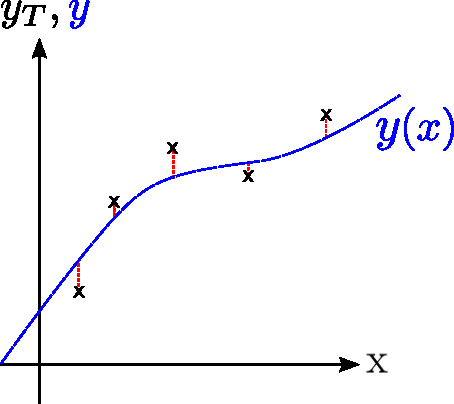
\includegraphics[height=4cm]{img/Regression_example}
    \end{center}
}
}
\only<2>{
    \begin{center}
        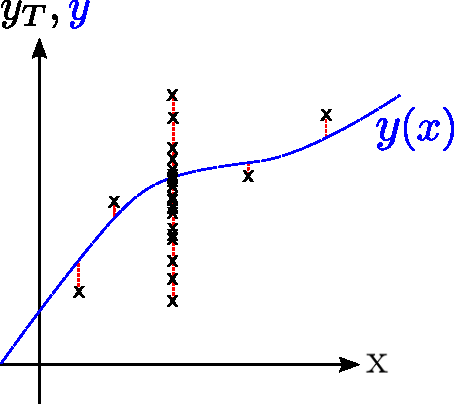
\includegraphics[height=4cm]{img/Regression_example_dense}
    \end{center}
}
\only<3>{
%\begin{figure}[h]
     %\centering
	%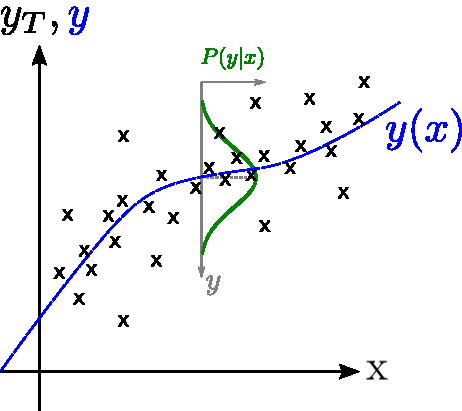
\includegraphics[width=0.4\textwidth]{img/gaussian_labels}
	%\caption{Gaussian distributed labels}
	%\label{fig:gaussian_labels}
%\end{figure}

\begin{figure}[ht]
     \centering
     \savebox{\imagebox}{
	 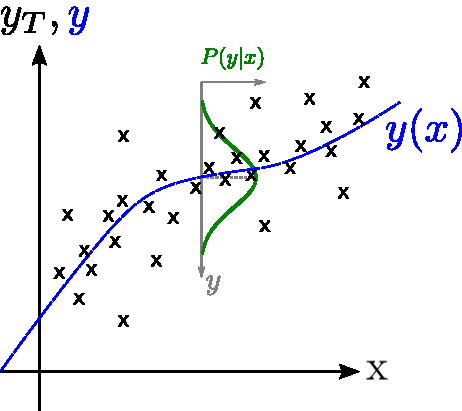
\includegraphics[width=0.37\textwidth]{img/gaussian_labels}}%
     \begin{subfigure}[t]{0.37\textwidth}
         \centering
         \usebox{\imagebox}% Place largest image
         \caption{guassian labels}
         \label{fig:quadratic}
     \end{subfigure}
     \hspace{2mm}
     \begin{subfigure}[t]{0.37\textwidth}
         \centering
         \raisebox{\dimexpr.5\ht\imagebox-.5\height}{% Raise smaller image into place
         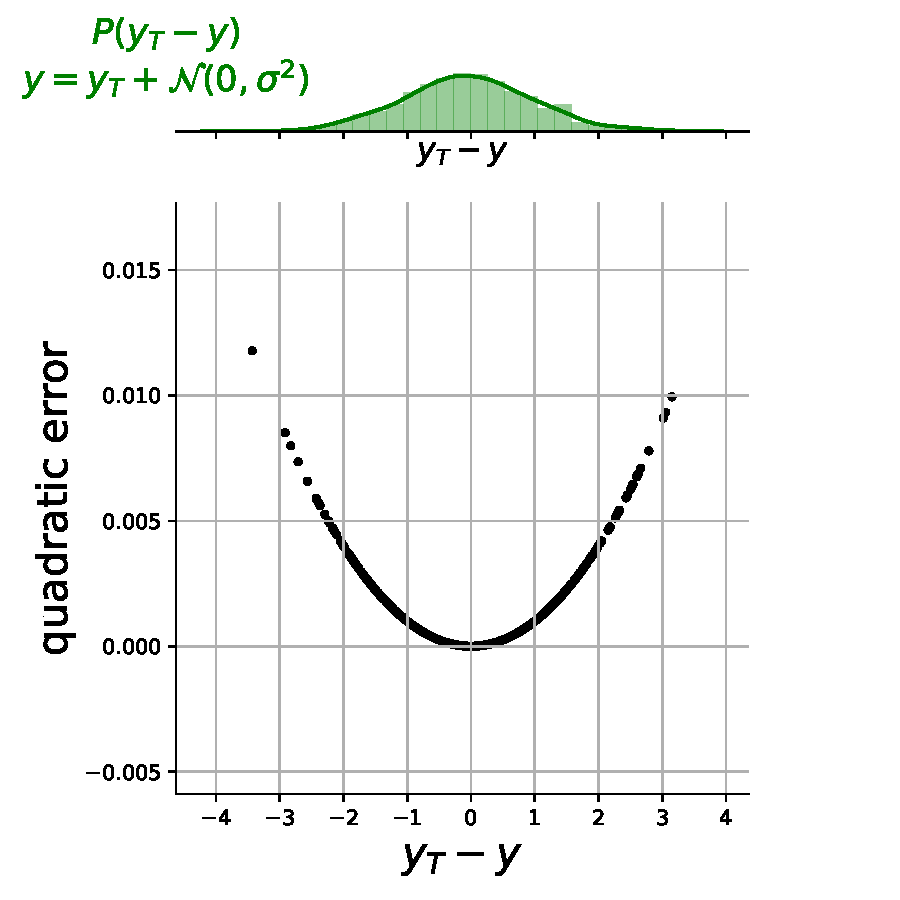
\includegraphics[width=0.99\textwidth]{img/qudaratic_conditional}
         }
         \caption{aggregate density}
         \label{fig:linear}
     \end{subfigure}
     \mode<article>{
     \caption{quadratic error and guassian labels}
     }
	 \label{fig:quadratic_density_gaussian}
\end{figure}
}
\only<4>{
\begin{align}
\vec w^* \in \argmin_{\vec w} \ETw 
\iff& 
\argmax_{\vec w} \underbrace{\prod_{\alpha=1}^{p} \mathcal{N}(y_T|{y(\vec x;\vec w)},\sigma^2)
}_{
\text{likelihood function } \mathcal{L(\vec w)}
}\\
&=
\argmin_{\vec w}
\underbrace{
 \lbrack - \ln \mathcal{L(\vec w)}\rbrack
 }_{\text{neg. log likelihood}}
\end{align} 
}


\end{frame}

\mode<article>{
This property makes the quadratic cost function the standard choice for regression.
}

\subsubsection{Cost functions for binary classification}

\begin{frame}\frametitle{\subsubsecname\\Deriving the cross entropy cost function for binary classification}

\mode<article>{
\textbf{Deriving the cross entropy cost function for binary classification}
}

\begin{itemize}
\item[]\underline{Data}:\\

\begin{equation}
\Big\{ \left( \vec x^{(\alpha)}, y_T^{(\alpha)} \right) \Big \}_{\alpha=1}^{p}
\end{equation}

with 
$$
\vec x^{(\alpha)} \in \R^N\;\;,\;\; y_T^{(\alpha)} \in \{{\color{red}0}, {\color{blue}1}\}.
$$

generated by
\begin{equation}
\left( \vec x^{(\alpha)}, y_T^{(\alpha)} \right) \stackrel{\iid}{\sim} P_{\text{data}}(\vec x, y)
\end{equation}

\pause

\item[]\underline{Model}:\\

MLP, scalar output \mode<article>{interpreted as probability that $y(\vec x; \vec w)=1$. In other words the probability of $\vec x$ belonging to class '1' (the positive class):}

\begin{equation}
y(\vec x;\vec w) =: P_{\text{model}} ({\color{blue}y=1}|\vec x;\vec w) \;\; \text{and} \;\; P_{\text{model}} ({\color{red}y=0}|\vec x; \vec w) = 1-y(\vec x;\vec w)
\end{equation}

for the \textcolor{blue}{``positive''} and \textcolor{red}{``negative''/``other''} class respectively.

\end{itemize}

\end{frame}

\begin{frame}\frametitle{Cost function derivation via minimization of \\the Kullback-Leibler divergence}

\mode<article>{
\textbf{The Kullback-Leibler divergence }

}

$\dkl(P||Q)$ is a measure of how much a probability distribution $P$ differs from another distribution $Q$.

\begin{align}
\dkl\left(\, P( z) ||\, Q( z) \,\right)
:= \int d  z \, P( z)
\ln 
\left( 
\frac{P(z)}{Q(z)}
\right)
\end{align}

\only<1>{
\begin{center}
	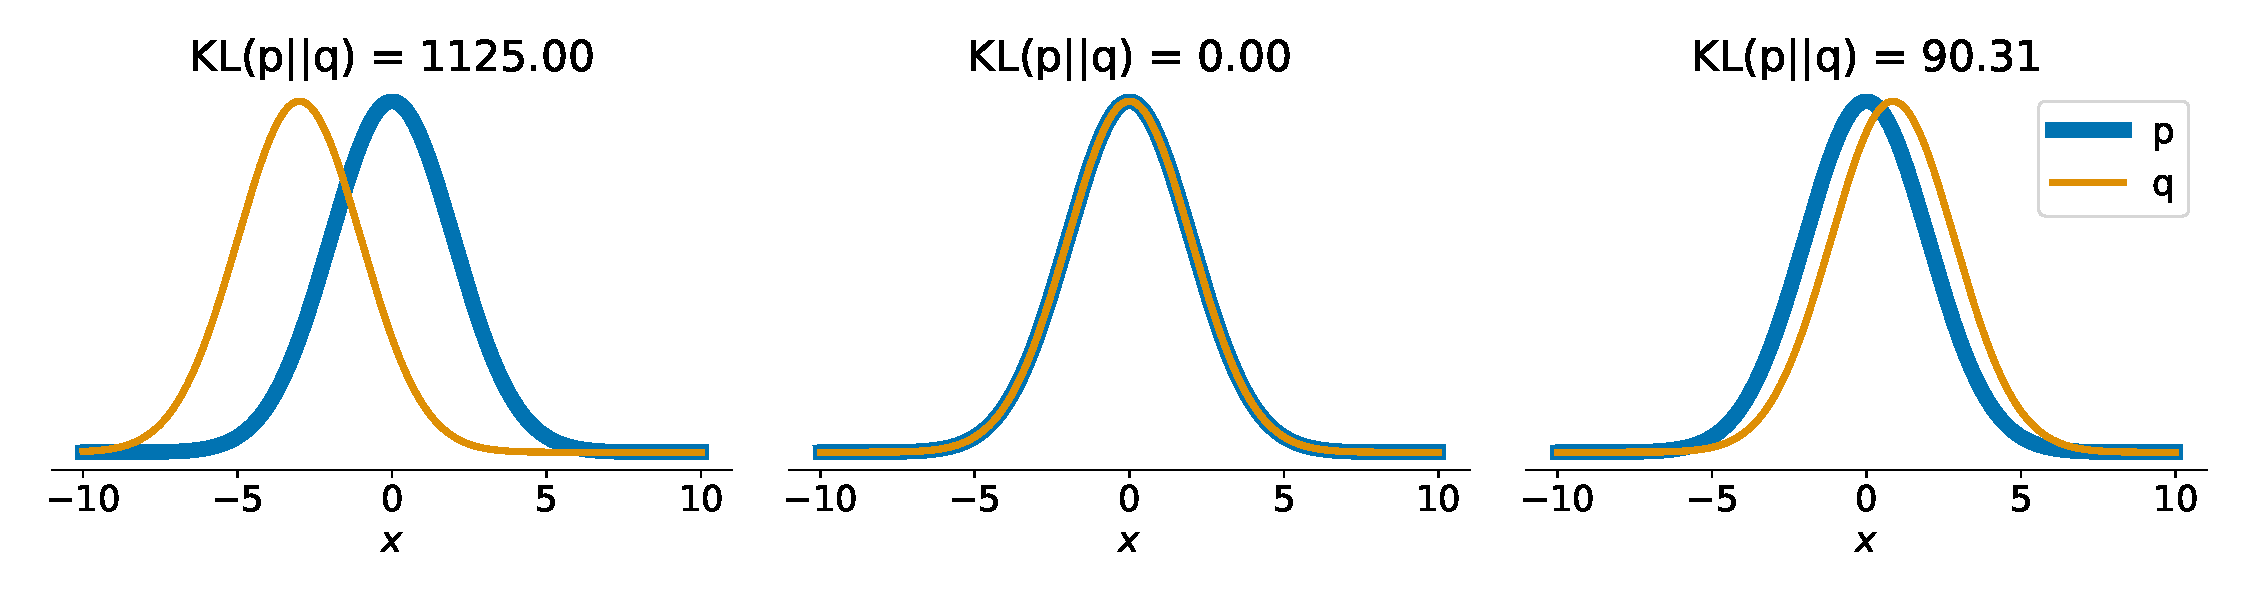
\includegraphics[width=0.7\textwidth]{img/kl_normal}
	\notesonly{\captionof{figure}{The KL divergence for comparing two distributions.}
	}
\end{center}
}
\only<2>{
Properties of the KL-divergence:

\begin{itemize}
\item $\dkl = 0$ iff. both distribution are \emph{identical},
\item otherwise, $\dkl > 0$.
\item[!] Does not qualify as a metric because it is not symmetric. For different distributions $P$ and $Q$:
	\begin{equation}
	\dkl(P||Q) \ne \dkl(Q||P)
	\end{equation}
\end{itemize}
}

\end{frame}

\begin{frame}\frametitle{Cost function derivation via minimization of the Kullback-Leibler divergence}
 
From KL-divergence to binary cross entropy loss:
\only<1>{

\begin{align}
\dkl\left(\, P_{\text{data}}(\vec x, y) \,||\, P_{\text{model}}(\vec x, y) \,\right)
= \iint d \vec x dy P_{\text{data}}(\vec x, y)
\ln 
\left( 
\frac{P_{\text{data}}(\vec x, y)}{P_{\text{model}}(\vec x, y)}
\right)
\end{align}

\mode<article>{
Integrating w.r.t. $y$ $\corresponds$ sum over the set of all possible values for $y$, which is $\{0,1\}$ in this case:
}
}
\definecolor{darkgreen}{rgb}{0,0.6,0}
\begin{align}
\only<1,2>{
\dkl&\left(\, P_{\text{data}}(\vec x, y) \,||\, P_{\text{model}}(\vec x, y) \,\right)\\
&= \int_{\R^N} d \vec x \sum_{y \in \{0,1\}} P_{\text{data}}(\vec x, y) \ln 
\left( 
\frac{P_{\text{data}}(\vec x, y)}{P_{\text{model}}(\vec x, y)}
\right)\\
}
\only<1,2>{
&= \int_{\R^N} d \vec x \sum_{y \in \{0,1\}} 
	\underbrace{
		P_{\text{data}}(\vec x)P_{\text{data}}(y | \vec x)
	}_{
		\substack{
		=P_{\text{data}}(\vec x, y)\\(\text{Bayes' rule})
		}
	}
	\ln 
	\left( 
		\frac{ P_{\text{data}}(\vec x)P_{\text{data}}(y | \vec x) }
		{
		\smash{
			\underbrace{
				P_{\hcancel[red]{\text{model}}}(\vec x)
				}_{
				\substack{
					\color{red}\text{discriminative model}\\
					\color{red}\text{not a generative model}\\
					\color{red}\text{replace with }
					{\color{cyan} P_{\text{data}}(\vec x)}
				}%substack
			}%underbrace
			\hspace{-5mm}
			P_{\text{model}}(y | \vec x)
		}%smash
		}%frac(lower)
	\right) \\
}
\only<2,3,4>{
&= \int_{\R^N} d \vec x \sum_{y \in \{0,1\}} 
	\underbrace{
		\color{darkgreen}
		P_{\text{data}}(\vec x)
	}_{\text{indep. of } y}
	P_{\text{data}}(y | \vec x)
	\ln 
	\left( 
	\frac{
		{ \color{cyan} P_{\text{data}}(\vec x) }
		{ \color{violet} P_{\text{data}}(y | \vec x) }
	}
	{
		{ \color{cyan} P_{\text{data}}(\vec x) }
		{ \color{brown} P_{\text{model}}(y | \vec x) }
	}%frac(lower)
	\right) \\
}
\only<3,4>{
&= \underbrace{
	\int_{\R^N} d \vec x \,
	{ \color{darkgreen} P_{\text{data}}(\vec x) }
	\sum_{y \in \{0,1\}}
	P_{\text{data}}(y | \vec x)
	\ln 
	\lbrack { \color{violet} P_{\text{data}}(y | \vec x) } \rbrack
	}_{\text{indep. of model parameters } \vec w} \\
	&\qquad- \int_{\R^N} d \vec x \,
		{ \color{darkgreen} P_{\text{data}}(\vec x) }
		\underbrace{
			\sum_{y \in \{0,1\}}
			P_{\text{data}}(y | \vec x)
			\ln
			\lbrack {\color{brown} P_{\text{model}}(y | \vec x) } \rbrack
		}_{
		\substack{
		\text{\textbf{cross entropy} between } \\
		\text{data \& model distributions given }\vec x}
		}
}
\end{align}

\mode<presentation>{
\only<4>{
Apply ERM on the second term with \textbf{cross entropy}.
}
}

\end{frame}

\begin{frame}\frametitle{ERM}

\mode<article>{
ERM for computing cross entropy loss using the training data:
}
\mode<presentation>{
\vspace{-5mm}
}

\begin{align}
\onslide<1->{
\ETw &= \frac{1}{p} \sum_{\alpha=1}^{p} - \bigg( \;
	\sum_{y\in\{{\color{red}0},{\color{blue}1}\}} P_{\text{data}}(y | \vec x^{(\alpha)})
	 \ln \lbrack P_{\text{model}}(y | \vec x^{(\alpha)}) \rbrack
	 \;\bigg)\\
	 &= \frac{1}{p} \sum_{\alpha=1}^{p} - \bigg( \;
	P_{\text{data}}({\color{blue}y=1} | \vec x^{(\alpha)})
	 \ln \lbrack P_{\text{model}}({\color{blue}y=1} | \vec x^{(\alpha)}) \rbrack \\
	 &\qquad\qquad\qquad+
	 P_{\text{data}}({\color{red}y=0} | \vec x^{(\alpha)})
	 \ln \lbrack P_{\text{model}}({\color{red}y=0} | \vec x^{(\alpha)}) \rbrack 
	  \;\bigg)\\
}
\onslide<2->{
	 &= \frac{1}{p} \sum_{\alpha=1}^{p} - \bigg( \;
		{\color{blue}y_T^{(\alpha)}} \cdot
	 \ln \lbrack {\color{blue}y(\vec x^{(\alpha)};\vec w)} \rbrack
	 + ( {\color{red}1-y_T^{(\alpha)}} ) \cdot
	 \ln \lbrack {\color{red}1-y(\vec x^{(\alpha)};\vec w)} \rbrack
	 \;\bigg)\\
}
\onslide<3->{
	 &= \frac{1}{p} \sum_{\alpha=1}^{p} \bigg( -
		{\color{blue}y_T^{(\alpha)}} \cdot
	 \ln \lbrack {\color{blue}y(\vec x^{(\alpha)};\vec w)} \rbrack
	 - ( {\color{red}1-y_T^{(\alpha)}} ) \cdot
	 \ln \lbrack {\color{red}1-y(\vec x^{(\alpha)};\vec w)} \rbrack  \;\bigg) \\
	 \notesonly{
	 &= \frac{1}{p} \sum_{\alpha=1}^{p} e\tyxwalpha
	 }
}
\end{align}

Extendable to multi-class cross entropy alongside \emph{softmax} normalization.

\end{frame}

\newpage

\begin{frame}
    
{
\notesonly{
\renewcommand{\arraystretch}{1.4} %<- control vertical spacing
}
\slidesonly{
\renewcommand{\arraystretch}{1.2} %<- control vertical spacing
}
\begin{center}
%\begin{table}[h!]
\notesonly{\captionof{table}{Cost functions \& output layers}\slidesonly{\vspace{-5mm}}}
\resizebox{0.9\textwidth}{!}{%
\hskip-2.0cm
\begin{tabular}{|l|c|c|l|}
\hline
task 
&  
\begin{tabular}[c]{@{}c@{}}\multicolumn{1}{c}
~\\[-5mm]
data\\
$\big\{ \vec x^{(\alpha)}, y_T^{(\alpha)} \big\}_{\alpha=1}^{p}$\\[2mm]
\end{tabular}
& output layer 
& \begin{tabular}[c]{@{}c@{}}
    cost function\\ 
    $e := e\tyxw$\end{tabular} \\ 
\hline \hline
scalar regression 
& 
$y_{T} \in \R$
& \begin{tabular}[c]{@{}l@{}}linear\\ $y = {\vec w^{LL-1}}^{\top} \vec s^{L-1}$\end{tabular} 
& \begin{tabular}[c]{@{}c@{}}quadratic error\\
$e = \frac{1}{2} \big( y_{T} - y\big)^{2}$\end{tabular} 
\pause
\\ \hline
\begin{tabular}[c]{@{}l@{}}multivariate linear \\ regression\end{tabular} 
&  
$\vec y_{T} \in \R^{M}$
& \begin{tabular}[c]{@{}l@{}}linear\\ $y_{k} = {\vec w_{k}^{LL-1}}^{\top} \vec s^{L-1}$\end{tabular} 
& \begin{tabular}[c]{@{}c@{}}squared Euclidean \\ distance\\ 
$e = \frac{1}{2} \lVert \vec y_{T} - \vec y \rVert^{2}_{2}$
\end{tabular}
\pause
\\ \hline
\begin{tabular}[c]{@{}l@{}}binary \\ classification\end{tabular} 
&  $y_{T} \in \{0,1\}, \{-1,1\}$
&
\begin{tabular}[c]{@{}c@{}}logistic sigmoid\\ 
$y = \frac{1}{1+exp(-h_{1}^{L})}$\\
or $y = \tanh(h_{1}^{L})$
\end{tabular} 
& \begin{tabular}[c]{@{}l@{}}cross entropy\\ 
$
e = \kern-.5ex
- y_T
\ln \lbrack y \rbrack \quad$\\
$
\;
-\kern-.2ex ( 1\kern-.5ex-\kern-.5exy_T )
\ln \lbrack 1\kern-.5ex-\kern-.5exy \rbrack
$
\end{tabular}
\pause
\\ \hline
\begin{tabular}[c]{@{}l@{}}multi-class \\ classification\\ with $M$ classes\end{tabular} 
&  
\begin{tabular}[c]{@{}c@{}}
$\vec {y}_{T} \in \{0,1\}^{M}$\\
1-out-of-$M$ encoding/\\
1-hot-encoding\\
e.g. $\vec {y}_{T}=(0,0,1,0)^{\top}$\\ $\corresponds$ class 3 out of 4
\end{tabular}
& \begin{tabular}[c]{@{}c@{}}softmax\\ 
$y_{k} = \frac{exp(h_{k}^{L})}{\sum_{k=1}^{M} exp(h_{k}^{L})}$\\[5mm]
$\Rightarrow \sum_{k=1}^{M} y_{k} = 1$
\end{tabular}
& \begin{tabular}[c]{@{}c@{}}cross entropy\\(multi-class case)\\ 
$
e = \kern-.3ex
-\kern-.2ex\sum_{k=1}^{M} {y_T}_{k} $\\
$\;\;\cdot 
%$\cdot
\ln \lbrack y_{k}\big(\vec x; \vec w\big) \rbrack
$
\end{tabular} \\
\hline
\end{tabular}
}
%\end{table}
\end{center}
} % arraystretch

\end{frame}

\mode*

\clearpage

\mode<article>
\subsection{From KL-divergence to the cross-entropy cost in numbers}

\subsubsection{First: The KL-divergence in numbers}

\definecolor{darkgreen}{rgb}{0,0.6,0}
\begin{align}
\dkl&\left(\, P_{\text{data}}(\vec x, y) \,||\, P_{\text{model}}(\vec x, y) \,\right)\\
&= \underbrace{
	\int_{\R^N} d \vec x \,
	{ \color{darkgreen} P_{\text{data}}(\vec x) }
	\sum_{y \in \{\textcolor{red}{0},\textcolor{blue}{1}\}}
	P_{\text{data}}(y | \vec x)
	\ln 
	\lbrack { \color{violet} P_{\text{data}}(y | \vec x) } \rbrack
	}_{\text{indep. of } \vec w~\Rightarrow~\text{treat as const. =}~c} \\
	&\qquad- \int_{\R^N} d \vec x \,
		{ \color{darkgreen} P_{\text{data}}(\vec x) }
			\sum_{y \in \{\textcolor{red}{0},\textcolor{blue}{1}\}}
			P_{\text{data}}(y | \vec x)
			\ln
			\lbrack {\color{brown} P_{\text{model}}(y | \vec x) } \rbrack\\
&= c \; - \int_{\R^N} d \vec x \,
		{ \color{darkgreen} P_{\text{data}}(\vec x) }
			\sum_{y \in \{\textcolor{red}{0},\textcolor{blue}{1}\}}
			P_{\text{data}}(y | \vec x)
			\ln
			\lbrack {\color{brown} P_{\text{model}}(y | \vec x) } \rbrack\\
&= c \; - \int_{\R^N} d \vec x \,
		{ \color{darkgreen} P_{\text{data}}(\vec x) }
		\Big\lbrack
			P_{\text{data}}(\textcolor{red}{y=0} | \vec x)
			\ln
			\lbrack {\color{brown} P_{\text{model}}(\textcolor{red}{y=0} | \vec x) } \rbrack\\
	&\qquad\qquad\qquad\qquad +
			P_{\text{data}}(\textcolor{blue}{y=1} | \vec x)
			\ln
			\lbrack {\color{brown} P_{\text{model}}(\textcolor{blue}{y=1} | \vec x) } \rbrack
		\Big\rbrack\\
&= c \; - \int_{\R^N} d \vec x \,
		{ \color{darkgreen} P_{\text{data}}(\vec x) }
			P_{\text{data}}(\textcolor{red}{y=0} | \vec x)
			\ln
			\lbrack {\color{brown} P_{\text{model}}(\textcolor{red}{y=0} | \vec x) } \rbrack\\
	&\qquad- \int_{\R^N} d \vec x \,
		{ \color{darkgreen} P_{\text{data}}(\vec x) }
			P_{\text{data}}(\textcolor{blue}{y=1} | \vec x)
			\ln
			\lbrack {\color{brown} P_{\text{model}}(\textcolor{blue}{y=1} | \vec x) } \rbrack
\end{align}

\begin{enumerate}
\item \textbf{Correctly} classifiying a single \textcolor{blue}{positive} sample:\\
	A \textcolor{blue}{positive} sample implies:
	\begin{itemize}
	\item $P_{\text{data}}(\textcolor{red}{y=0} | \vec x) = 0.01$
	\item $P_{\text{data}}(\textcolor{blue}{y=1} | \vec x) = 0.99$
	\end{itemize}
	A \textbf{correct} classification implies:
	\begin{itemize}
	\item ${\color{brown} P_{\text{model}}(\textcolor{red}{y=0} | \vec x) } = 0.2$
	\item ${\color{brown} P_{\text{model}}(\textcolor{blue}{y=1} | \vec x) } = 0.8$
	\end{itemize}
	Plugging it into the equation above. Only a single sample, so no integration:
	\begin{align}
\dkl
&= c \; -
		{ \color{darkgreen} P_{\text{data}}(\vec x) }
		\cdot
		0.01 \cdot 
			\ln(0.2)
		-
		{ \color{darkgreen} P_{\text{data}}(\vec x) }
		\cdot
		0.99 \cdot 
			\ln(0.8)\\
&= c \; +
		{ \color{darkgreen} P_{\text{data}}(\vec x) }
		\cdot
		\lbrack
		-0.01 \cdot 
			\ln(0.2)
		-0.99 \cdot 
			\ln(0.8)
		\rbrack\\
&= c \; +
		{ \color{darkgreen} P_{\text{data}}(\vec x) }
		\cdot
		\lbrack
		0.016 + 0.221
		\rbrack\\
&= c \; +
		{ \color{darkgreen} P_{\text{data}}(\vec x) }
		\cdot
		0.237
	\end{align}
\item \textbf{Misclassifiying} a single \textcolor{blue}{positive} sample:\\
	A \textcolor{blue}{positive} sample implies:
	\begin{itemize}
	\item $P_{\text{data}}(\textcolor{red}{y=0} | \vec x) = 0.01$
	\item $P_{\text{data}}(\textcolor{blue}{y=1} | \vec x) = 0.99$
	\end{itemize}
	A \textbf{misclassification} implies:
	\begin{itemize}
	\item ${\color{brown} P_{\text{model}}(\textcolor{red}{y=0} | \vec x) } = 0.7$
	\item ${\color{brown} P_{\text{model}}(\textcolor{blue}{y=1} | \vec x) } = 0.3$
	\end{itemize}
	Plugging it into the equation above. Only a single sample, so no integration:
	\begin{align}
\dkl
&= c \; -
		{ \color{darkgreen} P_{\text{data}}(\vec x) }
		\cdot
		0.01 \cdot 
			\ln(0.7)
		-
		{ \color{darkgreen} P_{\text{data}}(\vec x) }
		\cdot
		0.99 \cdot 
			\ln(0.3)\\
&= c \; +
		{ \color{darkgreen} P_{\text{data}}(\vec x) }
		\cdot
		\lbrack
		-0.01 \cdot 
			\ln(0.7)
		-0.99 \cdot 
			\ln(0.3)
		\rbrack\\
&= c \; +
		{ \color{darkgreen} P_{\text{data}}(\vec x) }
		\cdot
		\lbrack
		0.004 + 1.19
		\rbrack\\
&= c \; +
		{ \color{darkgreen} P_{\text{data}}(\vec x) }
		\cdot
		1.194
	\end{align}
\item[]
\begin{align}
\dkl(\text{correct classification})
&\;\;<\;\;
\dkl(\text{misclassification})\\
c \; +
		{ \color{darkgreen} P_{\text{data}}(\vec x) }
		\cdot
		0.237
&\;\;<\;\;
	c \; +
		{ \color{darkgreen} P_{\text{data}}(\vec x) }
		\cdot
		1.194
\end{align}
\end{enumerate}

\subsubsection{Second: binary cross-entropy in numbers}

binary cross-entropy for an indivudal sample:
\begin{equation}
e(y_T, y(\vec x;\vec w)) = 
-
{\color{blue}y_T} \cdot
	 \ln \lbrack {\color{blue}y(\vec x;\vec w)} \rbrack
	 - ( {\color{red}1-y_T} ) \cdot
	 \ln \lbrack {\color{red}1-y(\vec x;\vec w)} \rbrack 
\label{eq:bincrossentropysample}
\end{equation}

\begin{enumerate}
\item \textbf{Correctly} classifiying a single \textcolor{blue}{positive} sample:\\
	A \textcolor{blue}{positive} sample implies:
	\begin{itemize}
	\item $y_T = 1$
	\end{itemize}
	A \textbf{correct} classification implies:
	\begin{itemize}
	\item $y(\vec x;\vec w) = 0.8$
	\end{itemize}
	Plugging it into \eqref{eq:bincrossentropysample} above:
	\begin{align}
	e(1, 0.8)
	=& 
	-
	{\color{blue}1} \cdot
		 \ln \lbrack {\color{blue}0.8} \rbrack
		 - ( {\color{red}1-1} ) \cdot
		 \ln \lbrack {\color{red}1-0.8} \rbrack\\
	=& 
	-
		 \ln \lbrack {\color{blue}0.8} \rbrack
		 - ( {\color{red}0} ) \cdot
		 \ln \lbrack {\color{red}0.2} \rbrack\\
	=&\,0.223
	\end{align}	
\item \textbf{Misclassifying} a single \textcolor{blue}{positive} sample:\\
	A \textcolor{blue}{positive} sample implies:
	\begin{itemize}
	\item $y_T = 1$
	\end{itemize}
	A \textbf{wrong} classification implies:
	\begin{itemize}
	\item $y(\vec x;\vec w) = 0.3$
	\end{itemize}
	Plugging it into \eqref{eq:bincrossentropysample} above:
	\begin{align}
	e(1, 0.3)
	=& 
	-
	{\color{blue}1} \cdot
		 \ln \lbrack {\color{blue}0.3} \rbrack
		 - ( {\color{red}1-1} ) \cdot
		 \ln \lbrack {\color{red}1-0.3} \rbrack\\
	=& -
		 \ln \lbrack {\color{blue}0.3} \rbrack
		 - ( {\color{red}0} ) \cdot
		 \ln \lbrack {\color{red}0.7} \rbrack\\
	=&\,1.204
	\end{align}	
\item[]
\begin{align}
e(\text{correct})
&\;\;<\;\;
e(\text{wrong})\\
		0.223
&\;\;<\;\;
		1.204
\end{align}
\end{enumerate}

\mode*

\clearpage

\mode<all>
\section{Gradient-based learning}

\mode<presentation>{

\begin{frame}
\begin{center}
    \begin{center} \huge
        \secname
    \end{center}
    
    \begin{center}
		
\includegraphics[width=0.25\textwidth]{img/meme_slide}
    \end{center}
    
    \begin{center}
    Iterative, step-by-step minimization of the training error.
    \end{center}
\end{center}
\end{frame}
}

\begin{frame}\frametitle{Minimizing the training error}
	Training error $E^T$ for the training set $\left\{(\vec x^{(\alpha)}, y^{(\alpha)}_{T})\right\}$: 
    \begin{equation}
        \ETw = \frac{1}{p} \sum\limits_{\alpha = 1}^p 
					e\tyxwalpha
    \end{equation}
    
    \mode<article>{
    The objective is to minimize the training error w.r.t. the model parameters $\vec w$. That is
    }
    
    \begin{equation}
        \ETw \eqexcl \min_{\vec w} \quad \Rightarrow \quad \vec w^{*} = \argmin_{\vec w} \ETw
    \end{equation}

    \begin{figure}[h]
        \centering
        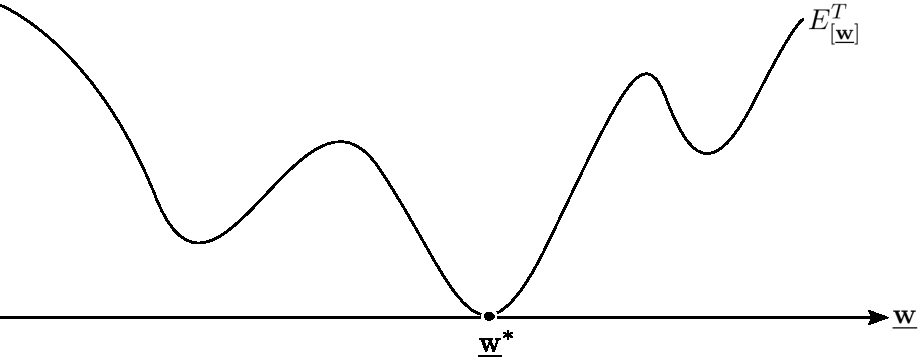
\includegraphics[height=2.5cm]{img/section1_fig19_no_steps}
        \caption{Training error with minimum at $\vec w^{*}$}
        \label{fig:training_error} 
    \end{figure}
    \slidesonly{\vspace{-10mm}}
    
    \pause 
    \question{What is the strategy for finding $\vec w^{*}$ analytically?}

\end{frame}

\subsection{Finding the minimum of the training error analytically}

\begin{frame}\frametitle{\subsecname}

    Example with a simple connectionist neuron model
    with parameters
    $$\vec w = (w_{0}, w_{1}, \ldots, w_{N})^{\top}$$\\


    - The strategy for finding the minimum of a function $\ETw$ analytically is as follows:
    \pause
    \begin{enumerate}
    \item Compute the gradient w.r.t. $\vec w$ by taking the first partial derivatives w.r.t to each component in the vector $\vec w$
    \begin{equation}
        \frac{\partial \ETw}{\partial \vec w} = \left(\,
        \frac{\partial \ETw}{\partial w_{0}}, \,
        \frac{\partial \ETw}{\partial w_{1}}, \,\ldots\,,\, 
        \frac{\partial \ETw}{\partial w_{N}}\,
        \right)^{\top}
        \label{eq:gradient_partial}
    \end{equation}
    The gradient $\frac{\partial \ETw}{\partial \vec w}$ has the same dimensionality as $\vec w$.
    \pause
    
    \item Set the gradient to zero: $\frac{\partial \ETw}{\partial \vec w} \eqexcl \vec 0$
    \item Solve for $\vec w$ to find extrema.
    \item Select solution corresponding to global minimum.
    
    \end{enumerate}
    
    Caveat: Closed-form solution infeasible for complex models such as MLPs.
    
    \mode<presentation>{
    Instead: Iterative learning algorithm gradient descent.
    }
\end{frame}

\subsection{Gradient descent}

\begin{frame}\frametitle{Finding the minumum of $\ETw$ iteratively\only<2->{ for an \underline{MLP}}}

\mode<article>{

Learning from gradient descent is an alternate approach for finding the minimum of a function when the closed-form solution is not available.

}
    \begin{figure}[h]
        \centering
        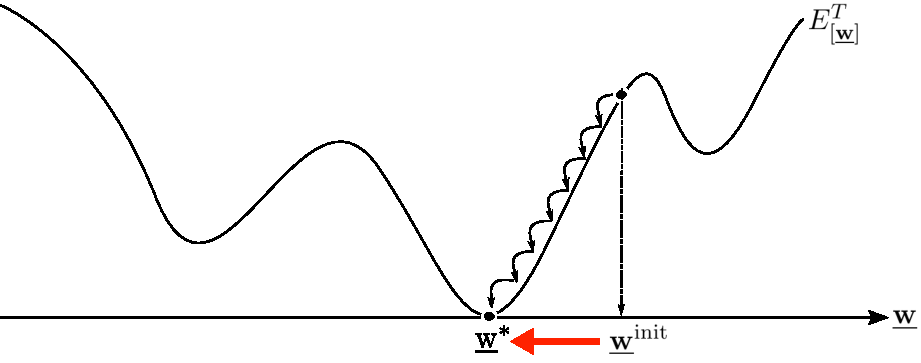
\includegraphics[height=3.cm]{img/section1_fig19}
        \caption{Minimizing the training error iteratively via gradient descent}
        \label{fig:minimize_via_gradient_descent} 
    \end{figure}
    
    \only<1>{
    For our connectionist neuron example:
    \begin{equation}
    		w_{j}(t+1) \quad=\quad w_{j}(t) 
				\;\;{\color{red}-}\;\;
				\underbrace{{\eta}}_{ 
						\substack{\text{learning} \\ \text{step} } }
                        \cdot
				\underbrace{\frac{\partial \ETw}{
					\partial {w}_{j}}}_{
						\substack{
							\text{component of}\\
							\text{\textcolor{red}{gradient vector}} 
			} }
            \label{eq:gradient_descent_neuron}
    \end{equation}
    
    with $j=0,\ldots,N$
    \mode<article>{
    $\vec w^{\mathrm{init}}$ is basically a random guess of where the solution might be and going against the gradient will potentially move us closer to the minimum. 
    }
    }
	\only<2,3>{
    For an MLP:
    \begin{equation}
		w_{ij}^{v'v}(t+1) \quad=\quad w_{ij}^{v'v}(t) 
				\;\;{\color{red}-}\;\;
				\underbrace{\eta}_{ 
						\substack{\text{learning} \\ \text{step} } }
                        \cdot
				\underbrace{\frac{\partial \ETw}{
					\partial {w}_{ij}^{v'v}}}_{
						\substack{
							\text{component of}\\
							\text{\textcolor{red}{gradient vector}} 
			} }
            \label{eq:gradient_descent_mlp}
    \end{equation}
    }
    
    \mode<article>{
    
    The learning step (learning rate) $\eta$ modulates the magnitude of our update. $\eta$ can be treated as a constant but we will also see how the value of $\eta$ can change over time, i.e. $\eta(t)$.
    }
    \only<3>{
    \mode<presentation>{\vspace{-4mm}}
    \question{Why do we \underline{subtract} the gradient from $w_{ij}^{v'v}(t)$?}
    }
    
    \mode<article>{
    
    The gradient describes the slope. Adding it will move us upwards and potentially maximize our function. Gradient-based learning with the intention of maximizing some function is referred to as hill climbing or gradient \emph{ascent}.
    }
    
    \only<4>{
    \question{So what's the downside of using gradient descent?}\\
    }
\end{frame}

\mode<article>{

    - The solution we find heavily depends on the initial position we started from. Indeed, gradient descent will reduce our cost each step but it does not guarantee that it will find the global minimum and will also stop at a local minimum. The slope in both cases is equal to zero.
    }

\begin{frame}\frametitle{\subsecname}
    
   \mode<presentation>{
    
    \textbf{So what's the downside of using gradient descent?}\\
    
    }
    
    \begin{figure}[h]
        \centering
        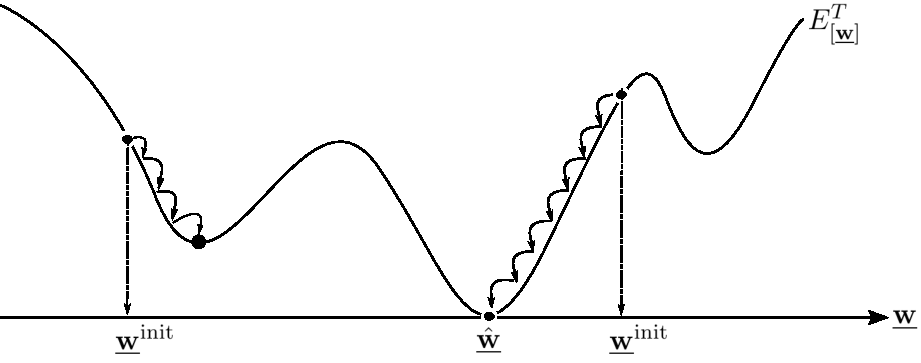
\includegraphics[height=3.25cm]{img/section1_fig19_local}
        \caption{Gradient descent finds local minima. We therefore denote the solution with $\hat{\vec w}$}
        \label{fig:minimize_via_gradient_descent_local} 
    \end{figure}
    
\end{frame}

\subsection{Gradient calculation: Connectionist neuron}

\begin{frame}\frametitle{Gradient calculation: Connectionist neuron}
    
    Recall the previous example with the connectionist neuron:
    
    \begin{figure}[h]
        \centering
        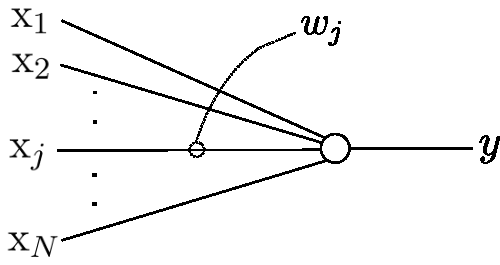
\includegraphics[height=2.5cm]{img/linearNeuron_y}
        \mode<article>{
        \caption{Connctionist neuron}
        }
        \label{fig:neuron} 
    \end{figure}
    
    Gradient descent updates the weights using:
    \begin{equation}
    		w_{j}(t+1) \quad=\quad w_{j}(t) 
				\;\;{\color{red}-}\;\;
				\underbrace{{\eta}}_{ 
						\substack{\text{learning} \\ \text{step} } }
                        \cdot
				\underbrace{\frac{\partial \ETw}{
					\partial {w}_{j}}}_{
						\substack{
							\text{component of}\\
							\text{\textcolor{red}{the gradient}} 
			} }
    \end{equation}
    
\end{frame}
\begin{frame}
    
    \only<1>{
    Knowing that
    \begin{align}
		\frac{\partial \ETw}
			{\partial {w}_{j}}
		\;&=\; \frac{1}{p} \sum_{\alpha=1}^p
        \frac{\partial e\tyxwalpha}
			{\partial {w}_{j}}
        =\; \frac{1}{p} \sum_{\alpha=1}^p 
        \frac{\partial e^{(\alpha)}}
			{\partial {w}_{j}}
	\end{align}
    }
    with $j=0,\ldots,N$.\\
    
    \mode<article>{
    The individual cost $e^{(\alpha)}$ is a function of terms that are functions of other terms themselves. Therefore, $\frac{\partial e^{(\alpha)}}{\partial {w}_{j}}$ is computed by applying the \emph{chain rule}:\\
    }
    \only<1,2>{
	\begin{equation}
		\frac{\partial \ETw}
			{\partial {w}_{j}}
		\;=\; \frac{1}{p} \sum_{\alpha=1}^p	\underbrace{
			\textcolor{blue}{
			\frac{\partial e\tyxwalpha}{\partial 
					y(\vec{x}^{(\alpha)}, \vec{w})} }}_{
						\substack{\text{factor depending} \\
							\text{on cost function}}}
				  \;\cdot \underbrace{
			\textcolor{orange}{
			\frac{\partial y(\vec{x}^{(\alpha)}; \vec{w})}{
					\partial {w}_{j}}} }_{
						\substack{\text{factor depending on} \\
							\text{model class}\\
                            \text{(e.g. perceptron, MLP)}}}
            \label{eq:gradient_terms}
	\end{equation}
    }
    
    \mode<article>{
    The first factor
    represents the first link from applying the chain rule. One recognizes that it only depends on the choice of the cost function. This \emph{error term} is completely independent of the type of model we choose.\\
    }
    
    \only<1>{
    \notesonly{
    Therefore, if the objective were to minimize} quadratic error:
    
    \mode<presentation>{\vspace{-1cm}}
    \begin{equation}
			e\tyxw := \frac{1}{2} \left( y_T - y(\vec{x}; \vec w) \right)^2
    \end{equation}
    
    \mode<article>{it follows:}
    
    \begin{equation}
			\textcolor{blue}{\frac{\partial e\tyxwalpha}{
					\partial y{(\vec{x}^{(\alpha)}; \vec{w})} }
				= - y_T^{(\alpha)} + y{(\vec{x}^{(\alpha)}; \vec{w})}}
    \end{equation}
    }
    
\mode<article>{
    The model-specific contribution to the error function appears in the second factor:
    
    Continuing with our connectionist neuron \notesonly{from \figref{fig:neuron}}:
    }

    \mode<presentation>{\vspace{-5mm}}
    \only<2>{
    \begin{equation}
            y(\vec x; \vec w) := 
            f \Big(\; \sum_{j=0}^{N} {w}_{j} {x}_j
            \; \Big){}
            = f \left( \vec w^{\top} \vec x\right)
            = f \left( h (\vec x; \vec w)\right)
    \end{equation}
    
    It follows:
    \begin{align}
			\textcolor{orange}{
			\frac{\partial y(\vec{x}^{(\alpha)}; \vec{w})}
            {\partial {w}_{j}}}
            &= \frac{\partial y(\vec{x}^{(\alpha)}, \vec{w})}
            {\partial h(\vec x^{(\alpha)}; \vec w)}
            \cdot
            \frac{\partial h(\vec x^{(\alpha)}; \vec w)}
            {\partial {w}_{j}}\\
            &= \underbrace{f'(h(\vec x^{(\alpha)}; \vec w))}_{\substack{\text{depends on}\\ \text{transfer function}}}
            \cdot
            \underbrace{
                \frac{\partial \vec w^{\top} \vec x^{(\alpha)}}
                {\partial {w}_{j}}
            }_{=x_{j}}
	\end{align}
    }
    
\end{frame}

\mode<presentation>{
\begin{frame}

	\begin{align}
		\frac{\partial \ETw}
			{\partial {w}_{j}}
		\;=\;& \frac{1}{p} \sum_{\alpha=1}^p	\underbrace{
			\textcolor{blue}{
			\frac{\partial e\tyxwalpha}{\partial 
					y(\vec{x}^{(\alpha)}, \vec{w})} }}_{
						\substack{\text{factor depending} \\
							\text{on cost function}}}
				  \;\cdot \underbrace{
			\textcolor{orange}{
			\frac{\partial y(\vec{x}^{(\alpha)}; \vec{w})}{
					\partial {w}_{j}}} }_{
						\substack{\text{factor depending on} \\
							\text{model class}\\
                            \text{(e.g. perceptron, MLP)}}}\\
            \;=\;& \frac{1}{p} \sum_{\alpha=1}^p
            \textcolor{blue}{(y{(\vec{x}^{(\alpha)}; \vec{w}) - y_T^{(\alpha)})}}
            \cdot
            \textcolor{orange}{
            \underbrace{f'(h(\vec x^{(\alpha)}; \vec w))}_{\substack{\text{depends on}\\ \text{transfer function}}}
            \cdot
            x_{j}
            }
	\end{align}

\begin{center}

\begin{minipage}{0.4\textwidth}
\begin{center}
	\includegraphics<2->[width=0.4\textwidth]{img/meme_perceptron_grad}
\end{center}
\end{minipage}
\begin{minipage}{0.4\textwidth}
\hspace{-30mm}
%\begin{center}
	%\includegraphics<3>[width=0.7\textwidth]{img/meme_showme_mlp}
    %\only<3>{img/meme_showme_mlp}
    %%%%%%%%%%%%%%%%%%%%%555
    %%%%%%%%%%%%%%%%%%%%%%5
    %%%%%%%%%%%%%%%%%%%%%%%55
    %%%%%%%%%%%%%%%%%%%%%%5
%\end{center}
\end{minipage}

\end{center}

\end{frame}
}

\begin{frame}\frametitle{Computing gradients for an MLP}

    \mode<presentation>{
    \begin{equation*}
        w_{ij}^{v'v}(t+1) \quad=\quad w_{ij}^{v'v}(t) 
            \;\;{\color{red}-}\;\;
            \underbrace{\eta}_{ 
                    \substack{\text{learning} \\ \text{step} } }
                    \cdot
            \underbrace{\frac{\partial \ETw}{
                \partial {w}_{ij}^{v'v}}}_{
                    \substack{
							\text{component of the }\\
                        \text{\textcolor{red}{gradient vector}} 
        } }
    \end{equation*}
    
    \begin{figure}[ht]
     \centering
     \savebox{\imagebox}{
	 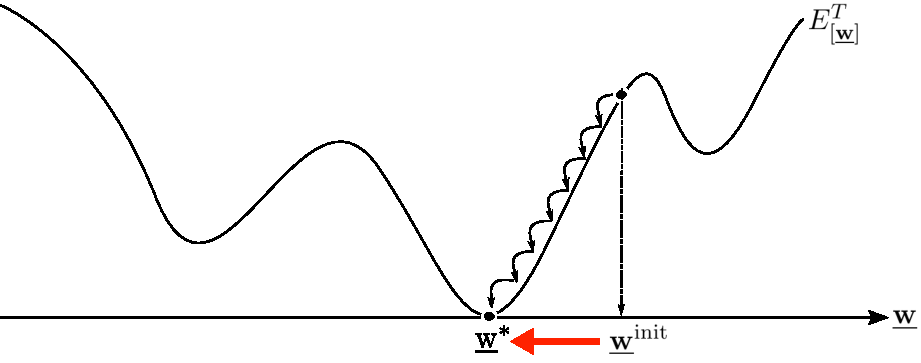
\includegraphics[trim=150 0 0 0,clip,height=2.5cm]{img/section1_fig19}}%
     \begin{subfigure}[t]{0.35\textwidth}
         \centering
         \usebox{\imagebox}% Place largest image
     \end{subfigure}
     \hspace{7mm}
     \begin{subfigure}[t]{0.49\textwidth}
         \centering
         \raisebox{\dimexpr.5\ht\imagebox-.5\height}{% Raise smaller image into place
         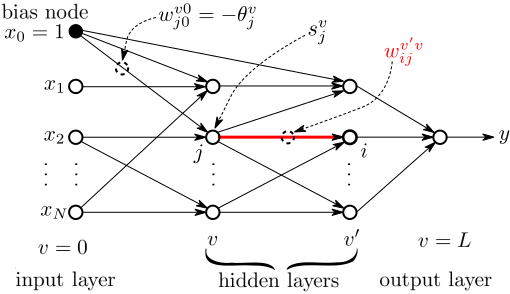
\includegraphics[width=0.99\textwidth]{img/section1_fig14_ij}
         }
     \end{subfigure}
    \end{figure}
    }
\end{frame}

    
    \mode<article>{
    \begin{figure}[h]
        \centering
        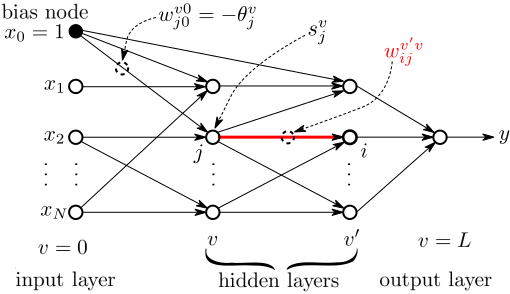
\includegraphics[height=3cm]{img/section1_fig14_ij}
        \caption{Example MLP architecture}
        \label{fig:example_mlp}
    \end{figure}
    
    \eqref{eq:gradient_descent_mlp} shows us how gradients are used for iteratively finding the minimum of the training error.
    The layered structure of an MLP implies that computing the gradient requires a more involved application of the chain rule. The backpropagation algorithm exploits the chain rule to efficiently compute the gradients for an MLP.
    }
    

\mode*

%\section{References}
%\begin{frame}[allowframebreaks] \frametitle{References}
	%\scriptsize
	%\bibliographystyle{plainnat}
	%\bibliography{bibliography}
%\end{frame}

\end{rightcolumn}
\end{paracol}

\end{document}
